\documentclass[12pt,twoside]{report}
% \documentclass[twoside]{report}
% Language setting
% Replace `english' with e.g. `spanish' to change the document language
\usepackage[USenglish]{babel}

% Set page size and margins
% Replace `letterpaper' with `a4paper' for UK/EU standard size
\usepackage[letterpaper,top=2cm,bottom=2cm,left=3cm,right=3cm,marginparwidth=1.75cm]{geometry}

% Useful packages
\usepackage{amsmath}
\usepackage{amssymb}
\usepackage{graphicx}
\usepackage{authblk}
\usepackage{times}
\usepackage{epsfig}
\usepackage{dcolumn}
\usepackage{bm}
\usepackage{color}
\usepackage{xcolor}
\usepackage{longtable}
\usepackage{array}
\usepackage{diagbox}
\usepackage{multirow}
\usepackage{enumerate}
\usepackage{booktabs}
\usepackage{stfloats}
\usepackage{fancyhdr}
\usepackage{feynmp-auto}
\usepackage[normalem]{ulem}
\usepackage{titlesec}
\usepackage{tocloft}
\usepackage{hyperref}
\hypersetup{
    colorlinks=true,
    linkcolor=blue,      % 设置内部链接(如目录项)的颜色
    citecolor=green,     % 设置引用的颜色
    filecolor=magenta,   % 设置文件链接的颜色
    urlcolor=black         % 设置网址链接的颜色
}
%%%%%%%%%%%%%%%%%%%%%%%%%%%%%%%%%%%%%%%%%%%%%%%%%%%%%%%%%%%%%%%
\newcommand{\tev}{\rm TeV}                     %  TeV
\newcommand{\gev}{\rm GeV}                     %  GeV
\newcommand{\gevc}{{\rm GeV}/c}                %  GeV/c
\newcommand{\gevcs}{{\rm GeV}/c^2}             %  GeV/c2
\newcommand{\mev}{\rm MeV}                     %  MeV
\newcommand{\mevcs}{{\rm MeV}/c^2}             %  MeV/c
\newcommand{\kev}{\rm KeV}                     %  KeV
\newcommand{\kevcs}{\kev/c^2}                  %  KeV/c2
\newcommand{\ev}{\rm eV}                       %  eV
\newcommand{\protonp}{p}
\newcommand{\pip}{\pi^+}      
\newcommand{\piz}{\pi^0}     
\newcommand{\pim}{\pi^-}
\newcommand{\kap}{K^+}
\newcommand{\kaz}{K^0}
\newcommand{\kam}{K^-}
\newcommand{\kabz}{\Bar{K}^0}
\newcommand{\kasp}{K^{*+}}
\newcommand{\kasz}{K^{*0}}
\newcommand{\kasm}{K^{*-}}
\newcommand{\kabsz}{\Bar{K}^{*0}}
\newcommand{\sigp}{\Sigma^+}
\newcommand{\sigz}{\Sigma^0}
\newcommand{\sigm}{\Sigma^-}
\newcommand{\kew}{\rm K}
\newcommand{\dd}{{\rm d}}
\newcommand{\rpip}{|\pip\rangle}
\newcommand{\rpiz}{|\piz\rangle}
\newcommand{\rpim}{|\pim\rangle}
%%%%%%%%%%%%%% Kaon %%%%%%%%%%%%%%%%%%%%
\newcommand{\rKap}{|\kap\rangle}
\newcommand{\rKaz}{|\kaz\rangle}
\newcommand{\rKam}{|\kam\rangle}
\newcommand{\rKabz}{|\kabz\rangle}
%%%%%%%%%%%%%% Kaon star %%%%%%%%%%%%%%%
\newcommand{\rKasp}{|\kasp\rangle}
\newcommand{\rKasz}{|\kasz\rangle}
\newcommand{\rKasm}{|\kasm\rangle}
\newcommand{\rKabsz}{|\kabsz\rangle}
\newcommand{\rpro}{|p\rangle}
\newcommand{\rneu}{|n\rangle}
\newcommand{\rprob}{|\Bar{p}\rangle}
\newcommand{\rneub}{|\Bar{n}\rangle}
%%%%%%%%%%%%%%%%%%%%%%%%%%%%%%%%%%%%%%%%%%%%%%%%%%%%%%%%%%%%%%%
\newcounter{problemname}
\numberwithin{problemname}{chapter}
\newenvironment{problem}{\vspace{1em}\stepcounter{problemname}\par\noindent {\large\textbf{\textsc{Problem \thechapter.\arabic{problemname}}}} \par\color{blue}}{\par}
\newenvironment{solution}{\vspace{1em}\par\noindent{\large\textbf{\textsc{Solution}}}\par}{\vspace{1em}\hrule}
%%%%%%%%%%%%%%%%%%%%%%%%%%%%%%%%%%%%%%%%%%%%%%%%%%%%%%%%%%%%%%%
\renewcommand{\thefootnote}{\fnsymbol{footnote}}

% \title{Solutions to Homework Problems from the \\{\it Particle Physics} Course Delivered by Ying Chen}
% \author[1,2]{Yan-Feng Li\thanks{E-mail: liyanfeng24@mails.ucas.ac.cn}}

% \affil[1]{Institute of High Energy Physics, Beijing 100049, China}
% \affil[2]{University of Chinese Academy of Sciences, Beijing 100049, China}

% \renewcommand*{\Affilfont}{\it}

% 设置章节标题居中
\titleformat{\chapter}[display]
  {\normalfont\huge\bfseries\centering} % 标题字体和大小,且居中
  {\chaptername\ \thechapter} % 章节编号
  {20pt} % 标题与章节内容的间距
  {\centering} % 标题居中
\renewcommand{\cftsecfont}{\large} % 段落标题的字体大小
\renewcommand{\cftsecpagefont}{\large} % 段落页码的字体大小
\renewcommand{\cftchapfont}{\Large} % 章节标题的字体大小
\renewcommand{\cftchappagefont}{\Large} % 章节页码的字体大小
%%%%%%%%%%%%%%%%%%%%%%%%%%%%%%%%%%%%%%%%%%%%%%%%%%%%%%%%%%%%%%%
\begin{document}
\begin{titlepage}
    \centering
    \href{https://www.ucas.ac.cn/}{
    \includegraphics[width=0.4\textwidth]{UCAS_LOGO.png}
    }\quad\quad
    \href{https://www.ihep.cas.cn/}{
    \includegraphics[width=0.53\textwidth]{IHEP_LOGO.png}
    }\\[0.8cm]
    % 学校名称
    {\Large \href{https://www.ucas.ac.cn/}{\textbf{\textsc{University of Chinese Academy of Sciences}}}} \\[0.2cm]
    {\Large \href{https://mooc.mooc.ucas.edu.cn/mooc-ans/course/350140000013013.html?clazzId=350140000017220}{\textbf{\textsc{particle physics, autumn 2024}}}} \\[5cm]

    % 标题
    {\LARGE \it \textbf{Solutions to Homework Problems from the \\[0.5cm] \href{https://mooc.mooc.ucas.edu.cn/mooc-ans/course/350140000013013.html?clazzId=350140000017220}{Particle Physics Course} Delivered by \href{https://people.ucas.edu.cn/~yingchen}{Ying CHEN}}} \\[1.5cm]

    % 作者信息
    {\Large Yan-Feng Li\footnote{E-mail: liyanfeng24@mails.ucas.ac.cn}} \\[0.5cm]

    % 机构
    {\large \it \href{https://www.ihep.cas.cn/}{Institute of High Energy Physics}, Beijing 100049, China} \\[0.2cm]
    {\large \it \href{https://www.ucas.ac.cn/}{University of Chinese Academy of Sciences}, Beijing 100049, China} \\[1cm]

    % 日期
    {\large \today}
\end{titlepage}
% \maketitle
\pagestyle{fancy}
\setlength{\headheight}{14.5pt}
\fancypagestyle{plain}{
    \fancyhf{}
    \fancyfoot[C]{-\enspace\thepage\enspace-}
    \renewcommand{\headrulewidth}{0pt}
}
\renewcommand{\headrulewidth}{0.4pt}
\pagenumbering{gobble}
\newpage
\pagenumbering{roman}
\tableofcontents
\newpage
\pagenumbering{arabic}
\setcounter{page}{1}
\fancyfoot{}
\fancyfoot[C]{-\enspace\thepage\enspace-}
%%%%%%%%%%%%%%%%%%%%%%%%%%%%%%%%%%%%%%%%%%%%%%%%%%%%%%%%%%%%%%%
\chapter{Basic Concepts and Kinematics}
\begin{problem}
What are the interaction ranges and typical interaction time of strong interaction, electromagnetic interaction and weak interaction? There are three unstable particles as follows: the width of particle $A$ is $100~\mev$, the width of particle $B$ is $5~\kev$, and the lifetime of particle $C$ is $3\times10^{-10}~{\rm s}$. Determine which interaction they mainly decay through.
\end{problem}

\begin{solution}
The effective range, interaction time and typical decay width of three interactions are listed in Table (\ref{tab:threeI}) showed below.
\begin{table}[ht]
\renewcommand{\arraystretch}{1.35}
\centering
\scalebox{1.2}{
\begin{tabular}{ccccc}
\toprule[1.5pt]
Interaction & Strong & EM & Weak \\\hline
Range & $1~{\rm fm}$ & $\infty$ & $1/400~{\rm fm}$\\
Time & $10^{-23}~{\rm s}$ & $\textcolor{red}{10^{-19}\sim} 10^{-16}~{\rm s}$ & $10^{-10}~{\rm s}$ \\
Width & $10\sim 100~\mev$ & $1~{\rm eV}$ & $10^{-6}~{\rm eV}$\\
\toprule[1.5pt]
\end{tabular}
}
\caption{\label{tab:threeI}Effective range, interaction time and typical width of three interactions.}
\end{table}
\par
Relation between width and lifetime is $\tau=\hbar/\Gamma$, $\hbar=6.57\times10^{-22}~{\rm MeV\cdot s}$ and we obtain $\tau_{A}=6.6\times10^{-24}~{\rm s}$ and $\tau_{B}=1.3\times10^{-19}~{\rm s}$. Therefore, A decays through strong interaction, \textcolor{red}{B decays by electromagnetic interaction} and C decays through weak interaction. \sout{As for particle B, its decay seems to be suppressed by rules like OZI rule, for instance, the $J/\psi$ as well as $\Upsilon$. For these particles mentioned above, it mainly decays through strong interaction}.
\end{solution}

\begin{problem}
Derive the Pauli-Schr\"{o}dinger Equation and deduce the magnetic moment of the electron. Start with the Dirac Equation in the presence of a external uniform magnetic field and perform a non-relativistic reduction.
\end{problem}

\begin{solution}
Dirac Equation has the form
\begin{equation}
    i\frac{\partial}{\partial t}\psi=(\mathbf{\alpha}\cdot\mathbf{p}+\beta m)\psi,\label{DiracEq}
\end{equation}
the $\mathbf{\alpha}$ and $\beta$ are $4\times4$ matrix which can be expressed as
\begin{equation}
    \mathbf{\alpha}=
    \begin{pmatrix}
        0 & \mathbf{\sigma} \\
        \mathbf{\sigma} & 0
    \end{pmatrix},
    \beta=
    \begin{pmatrix}
        \mathbf{I}_{2\times2} & 0 \\
        0 & -\mathbf{I}_{2\times2}
    \end{pmatrix}.
\end{equation}
$\mathbf{\sigma}$ is the Pauli Matrix.
\par
To Derive the magnetic moment of electron, we make use of the principle of minimal coupling and only focus on the time-independent case, then the Dirac Equation \eqref{DiracEq} turns to
\begin{equation}
    \begin{pmatrix}
        m & \bm{\sigma}\cdot\bm{\pi} \\
        \bm{\sigma}\cdot\bm{\pi} & -m
    \end{pmatrix}
    \begin{pmatrix}
        \psi_1 \\
        \psi_2
    \end{pmatrix}
    =E
    \begin{pmatrix}
        \psi_1 \\
        \psi_2
    \end{pmatrix},\label{Diracmatrix}
\end{equation}
where $\bm{\pi}=(\mathbf{p}-q\mathbf{A})$ and $\nabla\times\mathbf{A}=\mathbf{B}$.
\par
We rewrite energy as $E=m+\epsilon$, where $\epsilon$ is much smaller than $m$, to make a non-relativistic reduction. Then we can express $\psi_2$ in the form of $\psi_1$ according to Eq. \eqref{Diracmatrix}:
\begin{equation}
    \psi_2=\frac{\bm{\sigma}\cdot\bm{\pi}}{2m+\epsilon}\psi_1.\label{psi2}
\end{equation}
We can see that the numerator which has order of $\mathbf{p}\sim\mathcal{O}(\epsilon)$ is much smaller than denominator, which means $\psi_1$ dominate the wave-function $\psi$. Substitute $\psi_2$ with $\psi_1$ and drop out the $\epsilon$ in Eq. \eqref{psi2}, we obtain
\begin{equation}
    \frac{(\bm{\sigma}\cdot\bm{\pi})^2}{2m}\psi_1=\epsilon \psi_1.
\end{equation}
This is what is called Pauli-Schr\"{o}dinger Equation and $\epsilon$ is eigenvalue of this equation, we rewrite it as $E_{P}$.
\par
To simplify this equation, we can utilize the Pauli Matrix's property:
\begin{equation}
    \sigma^i\sigma^j=\delta^{ij}+i\epsilon^{ij}_{~~k}\sigma^k,
\end{equation}
and it makes
\begin{equation}
    (\bm{\sigma}\cdot\bm{\pi})^2=\sigma^i\pi_i\sigma^j\pi_j=\delta^{ij}\pi_i\pi_j+i\epsilon^{ij}_{~~k}\pi_i\pi_j\sigma^k=\bm{\pi}^2+i\bm{\sigma}\cdot(\bm{\pi}\times\bm{\pi}).
\end{equation}
Replace $\bm{\pi}$ with $\mathbf{p}-q\mathbf{A}$ and let $\mathbf{p}\to -i\nabla$, we have
\begin{equation}
    \bigg[\frac{(\mathbf{p}-q\mathbf{A})^2}{2m}-\frac{i\bm{\sigma}\cdot(\nabla-iq\mathbf{A})\times(\nabla-iq\mathbf{A})}{2m}\bigg]\psi_1=E_P \psi_1.
\end{equation}
The $\nabla\times(\mathbf{A\psi})=(\nabla\times\mathbf{A})\psi+\nabla\psi\times\mathbf{A}$, $\nabla\times\nabla=0$ and $\mathbf{A}\times\mathbf{A}=0$, thus it becomes
\begin{equation}
    \bigg[\frac{(\mathbf{p}-q\mathbf{A})^2}{2m}-\frac{q}{2m}\bm{\sigma}\cdot\mathbf{B}\bigg]\psi_1=E_P \psi_1.
\end{equation}
The $\frac{q}{2m}$ is the magnetic moment of the electron. Substitute $\bm{\sigma}$ with spin operator $\mathbf{S}=\frac{\bm{\sigma}}{2}$, introduce the Landé factor $g$ and ignore the subscript of $\psi$, we have
\begin{equation}
    \bigg[\frac{(\mathbf{p}-q\mathbf{A})^2}{2m}-g\frac{q}{2m}\mathbf{S}\cdot\mathbf{B}\bigg]\psi=E_P \psi.
\end{equation}
From this we know that the $g$ - factor of electron is $2$.
\end{solution}

\begin{problem}
Derive the mass distribution of an unstable particle whose mass and lifetime are $M_0$ and $\tau$.  
\end{problem}

\begin{solution}
Decay width of this particle is $\Gamma=1/\tau$. Suppose that the particle's state is $|t \rangle$, and it follows
\begin{equation}
    |t\rangle=e^{-i(M_0-i\Gamma)t}|0\rangle,
\end{equation}
where $|0\rangle$ is the initial state at $t=0$.
\par
To get the distribution with respect to mass $M$, we perform a Fourier transformation to $|t\rangle$
\begin{equation}
    |M\rangle=\int\frac{\dd t}{\sqrt{2\pi}}e^{iMt}|t\rangle=\frac{1}{\sqrt{2\pi}}\frac{i}{(M-M_0)+i\frac{\Gamma}{2}}|0\rangle.
\end{equation}
\par
The inner product of $|M\rangle$ gives distribution with respect to $M$:
\begin{equation}
    \langle M|M\rangle=\frac{1}{2\pi}\frac{1}{(M-M_{0})^2+\frac{\Gamma^2}{4}},
\end{equation}
and we have normalized $\langle 0|0\rangle$ to $1$.
\par Substitute $\Gamma$ with $1/\tau$, we obtain 
\begin{equation}
    f(M)=\frac{1}{2\pi}\frac{1}{(M-M_0)^2+\frac{1}{4\tau^2}}.
\end{equation}
\end{solution}

\begin{problem}
How to estimate an unstable particle's lifetime assuming that it can leave a trace in detector?
\end{problem}

\begin{solution}
The $x^{\mu}p_{\mu}$ is a Lorentz invariant, and it's same at center-of-mass frame and at laboratory frame:
\begin{equation}
    m\tau=Et-pL=E\frac{L}{v}-pL=E^2\frac{L}{p}-pL=\frac{L}{p}(E^2-p^2)=\frac{m^2L}{p},
\end{equation}
therefore, we have $\tau=Lm/p$.
\end{solution}

\begin{problem}
In a symmetric electron-positron collider, how fast does an electron need to collide to create a $J/\psi$ particle? What is the relative velocity of the electron and the positron? What about the rapidity and relative rapidity?
\end{problem}

\begin{solution}
The relationship between energy and mass of electron is
\begin{equation}
    E=\gamma m_e,
\end{equation}
where $\gamma=1/\sqrt{1-v^2}$ is the Lorentz factor. The energy of electron is $m_{J/\psi}/2=1.55~\gev$, thus we get
\begin{equation}
    v=0.999999945c.
\end{equation}
\par
The relative velocity of two particles $A$ and $B$ follows:
\begin{equation}
    v_{AB}=\frac{v_A+v_B}{1+v_{A}v_{B}},
\end{equation}
which gives that the relative velocity of the electron and the positron $v_r$ is almost equal to $c$ (fourteen nines behind the decimal point).
\par
Rapidity $y$ is defined with
\begin{equation}
    y=\frac{1}{2}\ln{\frac{1+v}{1-v}},
\end{equation}
therefore the rapidity of the electron is $y_{e^{-}}=8.7$. Rapidity is additive so the relative rapidity is $y_r=17.4$.
\end{solution}

\begin{problem}
Show that
\begin{equation}
    s+t+u=m_1^2+m_2^2+m_3^2+m_4^2,
\end{equation}
where $s,t$ and $u$ are Mandelstam variables:
\begin{align}
    s&=(p_1+p_2)^2=(p_3+p_4)^2 \\
    t&=(p_1-p_3)^2=(p_2-p_4)^2 \\
    u&=(p_1-p_4)^2=(p_2-p_3)^2.
\end{align}
\end{problem}

\begin{solution}
\begin{align}
    s+t+u&=(p_1+p_2)^2+(p_1-p_3)^2+(p_1-p_4)^2 \nonumber \\
    &=3m_1^2+m_2^2+m_3^2+m_4^2+2p_1p_2-2p_1p_3-2p_1p_4 \nonumber \\
    &=3m_1^2+m_2^2+m_3^2+m_4^2+2p_1(p_2-p_3-p_4) \nonumber \\
    &=3m_1^2+m_2^2+m_3^2+m_4^2-2p_1^2 \nonumber \\
    &=m_1^2+m_2^2+m_3^2+m_4^2,
\end{align}
where we have used the condition that the four-momentum should conserve ($p_1+p_2=p_3+p_4$).
\end{solution}

\begin{problem}
Derive the formula of three-body decay width and explain the physical meaning of Dalitz plot.
\end{problem}

\begin{solution}
Differential decay width is written as:
\begin{equation}
    \dd \Gamma=|\mathcal{M}|^2\dd \Phi_n,
\end{equation}
where $\mathcal{M}$ is amplitude and $\Phi_n$ is $n$-body phase space
\begin{equation}
    \dd \Phi_n=(2\pi)^4\delta^4(P-P_f)\frac{1}{2M} \prod_{i=1}^{n}\frac{\dd^3\mathbf{p_i}}{(2\pi)^3}\frac{1}{2E_i},
\end{equation}
where $P$ is four-momentum of initial particle with mass $M$, $p_i=(E_i, \mathbf{p_i})$ are referred as four-momentum of daughter particles and $P_f$ is the sum of $p_i$.
\par
To calculate three-body decay width, we need to integrate the $\dd\Gamma$:
\begin{align}
    \Gamma&=\frac{1}{(2\pi)^5}\frac{1}{16M}\int |\mathcal{M}|^2\delta^4(P-p_1-p_2-p_3) \prod_{i=1}^{3}\dd^3\mathbf{p_i}\frac{1}{E_i} \nonumber \\
    &=\frac{1}{(2\pi)^5}\frac{1}{16M}\int |\mathcal{M}|^2\delta(M-E_1-E_2-E_3) \frac{\dd^3\mathbf{p_1}\dd^3\mathbf{p_2}}{E_1E_2E_3}.
\end{align}
According to $E_i^2=\mathbf{p_i}^2+m_i^2$, we have
\begin{equation}
    E_i\dd E_i=|\mathbf{p_i}|\dd|\mathbf{p_i}|,
\end{equation}
thus $\Gamma$ becomes
\begin{equation}
    \Gamma=\frac{1}{(2\pi)^5}\frac{1}{16M}\int |\mathcal{M}|^2\delta(M-E_1-E_2-E_3) \frac{|\mathbf{p_1}||\mathbf{p_2}|\dd E_1\dd E_2\dd \Omega_1\dd \Omega_2}{E_3}. \label{Eq:GammaInte}
\end{equation}
Here we have used spherical coordinates to represent the measure of integration \begin{equation}
    \dd^3 \mathbf{p}=|\mathbf{p}|^2\sin{\theta}\dd|\mathbf{p}|\dd\theta\dd\phi=|\mathbf{p}|\dd|\mathbf{p}|\dd\Omega.
\end{equation}
$\theta_2$ in Eq. \eqref{Eq:GammaInte} is the relative polar angle of $\mathbf{p_2}$ and $\mathbf{p_1}$.
\par
The $\delta$-function in Eq. \eqref{Eq:GammaInte} can be expressed as
\begin{equation}
    \delta(M-E_1-E_2-E_3)=\delta(\theta_2-\theta_2^*)\frac{1}{|\frac{\partial E_3}{\partial \theta_2}|},
\end{equation}
where $\theta_2^*$ is the value that makes $M-E_1-E_2-E_3=0$. $E_3$ can be written as
\begin{align}
    E_3&=\sqrt{\mathbf{p_3}^2+m_3^2} \nonumber \\
    &=\sqrt{(\mathbf{p_1}+\mathbf{p_2})^2+m_3^2} \nonumber \\
    &=\sqrt{\mathbf{p_1}^2+\mathbf{p_2}^2+2|\mathbf{p_1}||\mathbf{p_2}|\cos{\theta_2}+m_3^2},
\end{align}
thus we have
\begin{equation}
    \bigg|\frac{\partial E_3}{\partial \theta_2}\bigg|=\frac{|\mathbf{p_1}||\mathbf{p_2}|\sin{\theta_2}}{E_3}.
\end{equation}
\par
Therefore,
\begin{align}
    \Gamma&=\frac{1}{(2\pi)^5}\frac{1}{16M}\int |\mathcal{M}|^2\frac{E_3\delta(\theta_2-\theta_2^*)\dd\theta_2}{|\mathbf{p_1}||\mathbf{p_2}|\sin{\theta_2^*}}\frac{|\mathbf{p_1}||\mathbf{p_2}|\sin{\theta_2}}{E_3} \dd E_1\dd E_2\dd \Omega_1\dd\phi_2. \nonumber \\
    &=\frac{1}{(2\pi)^3}\frac{1}{8M}\int|\mathcal{M}|^2\dd E_1\dd E_2. \label{E1E2Form}
\end{align}
Define Lorentz invariant $m_{23}$ and $m_{13}$:
\begin{align}
    m_{23}^2&=(p_2+p_3)^2=(P-p_1)^2=M^2+m_1^2-2ME_1, \nonumber \\
    m_{13}^2&=(p_1+p_3)^2=(P-p_2)^2=M^2+m_2^2-2ME_2.
\end{align}
Thus we have 
\begin{align}
    \dd E_1=-\frac{1}{2M}\dd m_{23}^2, \nonumber \\
    \dd E_2=-\frac{1}{2M}\dd m_{13}^2.
\end{align}
Substitute the $E_1$ and $E_2$ with $m_{23}$ and $m_{13}$ in Eq. \eqref{E1E2Form}, we have
\begin{equation}
    \Gamma=\frac{1}{(2\pi)^3}\frac{1}{32M^3}\int|\mathcal{M}|^2\dd m_{13}^2\dd m_{23}^2.
\end{equation}
To be more clear, we write it in the differential form:
\begin{equation}
    \frac{\dd^2\Gamma}{\dd m_{13}^2\dd m_{23}^2}=\frac{1}{(2\pi)^3}\frac{1}{32M^3}|\mathcal{M}|^2. \label{DiffDalitz}
\end{equation}
We know that event number $N$ is proportional to $\Gamma$. Eq. \eqref{DiffDalitz} shows that the 2-Dimension distribution of $N$ with respect to $m_{13}^2$ and $m_{23}^2$ gives an insight to $|\mathcal{M}|^2$ directly, and this kind of figure is named with the so-called {\it Dalitz Plot}. An example of Dalitz plot is showed in Fig. \ref{fig:Dalitz}. If $|\mathcal{M}|^2$ is a constant, $N$ should follow uniform distribution. Otherwise, a great number of events will be concentrated on certain $m_{13}^2$ or $m_{23}^2$ or both.
\begin{figure}
\centering
\includegraphics[width=0.90\textwidth]{dalitz.pdf}
\caption{\label{fig:Dalitz} A Dalitz plot for a three-body final state cited from PDG. In this example, the state is $\pip \bar{K^0} p$ at
3 GeV. Four-momentum conservation restricts events to the shaded region.}
\end{figure}
\end{solution}

\begin{problem}
Explain the relationships between luminosity ($L$), cross section ($\sigma$) and event number ($N$) as well as the meanings of them in High Energy Physics.
\end{problem}

\begin{solution}
The mathematical relationship between them is
\begin{equation}
    N=\sigma Lt,
\end{equation}
where the $N$ is a quantity that experiment physicist are mainly concerned with, it shows the expected number of events which should be observed in experiments. Cross section $\sigma$ reflects the physical dynamics in the process and it reveals mystery of the fundamental interactions. As for the luminosity $L$, it's an important parameter that shows how much data or events the collider can produce in unit time. Time is represented by $t$.
\end{solution}

\chapter{Symmetry and Conservation}
\begin{problem}
What are isospin and isospin transformation? Explain the meaning of isospin symmetry.
\end{problem}

\begin{solution}
\textbf{Isospin} is a quantum number which is used to describe strong interaction symmetry of the baryon. Mathematically, it follows the SU(2) transformation, which is similar to the spin. In strong interaction, isospin is the conserved charge under isospin transformations. 
\par
\textbf{Isospin transformation} is transforming a state in an isospin multiplet to another state at the same multiplet and it can be expressed by SU(2) group in mathematics.
\par
\textbf{Isospin symmetry} shows that if an interaction processes with strong force then this process should not be related to the charge of each particles involved in this interaction, that is, once we apply an isospin transformation to a strong process, the new process should have the same amplitude with the former one. Besides, isospin symmetry causes the conservation of isospin in strong interaction.
\end{solution}


\begin{problem}
What are the properties of strange particles? Why?
\end{problem}

\begin{solution}
1) \textbf{Produced coherently and decay independently}. Each strange particles carries strangeness and this quantity is a conservation charge under strong interaction. Therefore, when strange particles are produced, there should be at least two strange particles produced together and then each of them decays independently. \par
2) \textbf{Produced rapidly and decay slowly}. Strange particles are produced by strong interaction and the typical interaction time of strong force is about $10^{-24}$ s, while these strange particles are usually the lightest strange particles and they have to decay into normal particles via weak interaction which not conserves strangeness, and the typical interaction time of weak interaction is about $10^{-10}$ s.
\end{solution}

\begin{problem}
The pion system $(\pip,\piz,\pim)$ forms an isospin triplet, for
\begin{equation}
    |\pip\rangle=|1,1\rangle,\quad|\piz\rangle=|1,0\rangle,\quad|\pim\rangle=|1,-1\rangle, \nonumber
\end{equation}
and the nucleon system $N=\begin{pmatrix} p \\ n \\ \end{pmatrix}$ forms an isospin doublet:
\begin{equation}
    |p\rangle=|\frac{1}{2},\frac{1}{2}\rangle,\quad|n\rangle=|\frac{1}{2},-\frac{1}{2}\rangle, \nonumber
\end{equation}
while anti-nucleon system $\Bar{N}=\begin{pmatrix} \Bar{n} \\ -\Bar{p} \\ \end{pmatrix}$ forms another isospin doublet:
\begin{equation}
    |\Bar{n}\rangle=|\frac{1}{2},\frac{1}{2}\rangle,\quad-|\Bar{p}\rangle=|\frac{1}{2},-\frac{1}{2}\rangle, \nonumber
\end{equation}
the same formation is applied to $K$ meson doublet $K=\begin{pmatrix} K^+ \\ K^0 \\ \end{pmatrix}$ with strangeness $S=+1$ and $\Bar{K}=\begin{pmatrix} \Bar{K^0} \\ -K^- \\ \end{pmatrix}$ with strangeness $S=-1$, where
\begin{align}
    &|K^+\rangle=|\frac{1}{2},\frac{1}{2}\rangle,\quad|K^0\rangle=|\frac{1}{2},-\frac{1}{2}\rangle, \nonumber \\
    &|\Bar{K^0}\rangle=|\frac{1}{2},\frac{1}{2}\rangle,\quad-|K^-\rangle=|\frac{1}{2},-\frac{1}{2}\rangle. \nonumber
\end{align}
Find all the isospin states that can be formed by $\pi\pi$, $K\Bar{K}$, $NN$ and $N\Bar{N}$ in the expression of particles constitution and give the baryon number and strangeness of these systems.
\end{problem}

\begin{figure}
\centering
\includegraphics[width=1.1\textwidth]{CG_Coefficient.pdf}
\caption{\label{fig:CGCoefficient} Clebsch-Gordan coefficients cited from PDG.}
\end{figure}

\begin{solution}
For $\pi\pi$ system, the possible combinations of states are $|0,0\rangle$, $|1,0\rangle$, $|2,0\rangle$, $|1,1\rangle$, $|2,1\rangle$, $|1,-1\rangle$, $|2,-1\rangle$, $|2,2\rangle$ and $|2,-2\rangle$. According to the $1\times1$ C-G coefficients, we have
\begin{align*}
    |0, 0\rangle&=\sqrt{\frac{1}{3}}\rpip\rpim-\sqrt{\frac{1}{3}}\rpiz\rpiz+\sqrt{\frac{1}{3}}\rpim\rpip, \\
    |1,0\rangle&=\sqrt{\frac{1}{2}}\rpip\rpim-\sqrt{\frac{1}{2}}\rpim\rpip, \\
    |2,0\rangle&=\sqrt{\frac{1}{6}}\rpip\rpim+\sqrt{\frac{2}{3}}\rpiz\rpiz+\sqrt{\frac{1}{6}}\rpim\rpip, \\
    |1,1\rangle&=\sqrt{\frac{1}{2}}\rpip\rpiz-\sqrt{\frac{1}{2}}\rpiz\rpip, \\
    |2,1\rangle&=\sqrt{\frac{1}{2}}\rpip\rpiz+\sqrt{\frac{1}{2}}\rpiz\rpip, \\
    |1,-1\rangle&=\sqrt{\frac{1}{2}}\rpiz\rpim-\sqrt{\frac{1}{2}}\rpim\rpiz, \\
    |2,-1\rangle&=\sqrt{\frac{1}{2}}\rpiz\rpim+\sqrt{\frac{1}{2}}\rpim\rpiz, \\
    |2,2\rangle&=\rpip\rpip\quad\text{and}\quad|2,-2\rangle=\rpim\rpim. \\
\end{align*} \par
For $K\Bar{K}$ system, the possible combinations of states are $|0,0\rangle$, $|1,0\rangle$, $|1,1\rangle$, $|1,-1\rangle$. According to the $\frac{1}{2}\times\frac{1}{2}$ C-G coefficients, we have
\begin{align*}
    |0,0\rangle&=\sqrt{\frac{1}{2}}(|\frac{1}{2},\frac{1}{2}\rangle|\frac{1}{2},-\frac{1}{2}\rangle-|\frac{1}{2},-\frac{1}{2}\rangle|\frac{1}{2},\frac{1}{2}\rangle) \\
    &=\sqrt{\frac{1}{2}}(\rKap\rKam+\rKaz\rKabz), \\
    |1,0\rangle&=\sqrt{\frac{1}{2}}(|\frac{1}{2},\frac{1}{2}\rangle|\frac{1}{2},-\frac{1}{2}\rangle+|\frac{1}{2},-\frac{1}{2}\rangle|\frac{1}{2},\frac{1}{2}\rangle) \\
    &=\sqrt{\frac{1}{2}}(\rKap\rKam-\rKaz\rKabz), \\
    |1,1\rangle&=|\frac{1}{2},\frac{1}{2}\rangle|\frac{1}{2},\frac{1}{2}\rangle=\rKap\rKabz, \\
    |1,-1\rangle&=|\frac{1}{2},-\frac{1}{2}\rangle|\frac{1}{2},-\frac{1}{2}\rangle=\rKaz\rKam,
\end{align*}
where the overall sign has been dropped off. \par
For $NN$ system, the possible combinations of states are $|0,0\rangle$, $|1,0\rangle$, $|1,1\rangle$, $|1,-1\rangle$. According to the $\frac{1}{2}\times\frac{1}{2}$ C-G coefficients, we have
\begin{align*}
    |0,0\rangle&=\sqrt{\frac{1}{2}}(|\frac{1}{2},\frac{1}{2}\rangle|\frac{1}{2},-\frac{1}{2}\rangle-|\frac{1}{2},-\frac{1}{2}\rangle|\frac{1}{2},\frac{1}{2}\rangle) \\
    &=\sqrt{\frac{1}{2}}(\rpro\rneu-\rneu\rpro), \\
    |1,0\rangle&=\sqrt{\frac{1}{2}}(|\frac{1}{2},\frac{1}{2}\rangle|\frac{1}{2},-\frac{1}{2}\rangle+|\frac{1}{2},-\frac{1}{2}\rangle|\frac{1}{2},\frac{1}{2}\rangle) \\
    &=\sqrt{\frac{1}{2}}(\rpro\rneu+\rneu\rpro), \\
    |1,1\rangle&=|\frac{1}{2},\frac{1}{2}\rangle|\frac{1}{2},\frac{1}{2}\rangle=\rpro\rpro, \\
    |1,-1\rangle&=|\frac{1}{2},-\frac{1}{2}\rangle|\frac{1}{2},-\frac{1}{2}\rangle=\rneu\rneu.
\end{align*}
\par
For $N\Bar{N}$ system, the possible combinations of states are $|0,0\rangle$, $|1,0\rangle$, $|1,1\rangle$, $|1,-1\rangle$. According to the $\frac{1}{2}\times\frac{1}{2}$ C-G coefficients, we have
\begin{align*}
    |0,0\rangle&=\sqrt{\frac{1}{2}}(|\frac{1}{2},\frac{1}{2}\rangle|\frac{1}{2},-\frac{1}{2}\rangle-|\frac{1}{2},-\frac{1}{2}\rangle|\frac{1}{2},\frac{1}{2}\rangle) \\
    &=\sqrt{\frac{1}{2}}(\rpro\rprob+\rneu\rneub), \\
    |1,0\rangle&=\sqrt{\frac{1}{2}}(|\frac{1}{2},\frac{1}{2}\rangle|\frac{1}{2},-\frac{1}{2}\rangle+|\frac{1}{2},-\frac{1}{2}\rangle|\frac{1}{2},\frac{1}{2}\rangle) \\
    &=\sqrt{\frac{1}{2}}(\rpro\rprob-\rneu\rneub), \\
    |1,1\rangle&=|\frac{1}{2},\frac{1}{2}\rangle|\frac{1}{2},\frac{1}{2}\rangle=\rpro\rneub, \\
    |1,-1\rangle&=|\frac{1}{2},-\frac{1}{2}\rangle|\frac{1}{2},-\frac{1}{2}\rangle=\rneu\rprob,
\end{align*}
where the overall sign has been dropped off.\par
Both the pions and nuclei have no strangeness, so the strangeness of $\pi\pi$, $NN$ and $N\Bar{N}$ are zero. The strangeness of $K$ is $+1$ and which of $\Bar{K}$ is $-1$, therefore the total strangeness of $K\Bar{K}$ system is zero as well.
\par
Pions and kaons have no baryon number, so the baryon number of $\pi\pi$ and $K\Bar{K}$ are zero. The baryon number of $N$ is $+1$ and which of $\Bar{N}$ is $-1$, therefore the total strangeness for $N\Bar{N}$ system is zero and for $NN$ is 2.
\end{solution}

\begin{problem}
How much momentum is needed for a proton to collide with a proton target to create an anti-proton in the laboratory frame? ($m_{p}=1~\gevcs$)
\end{problem}

\begin{solution}
To keep the conservation of baryon number and charge, the process is written as
\begin{equation*}
    p+p\to p+p+p+\Bar{p}\ .
\end{equation*}
Let the four-momentum of beam proton $p_{b}=(E,\mathbf{p})$ and that of the target proton $p_{t}=(m_{p},0)$. The minimal momentum of $p_{b}$ is reached if the final four (anti-)protons are at rest at the center-of-mass frame and we donate the total four momentum of final state as $P_{f}$, where $P_{f}^2=16m_{p}^2$, therefore, we have
\begin{align*}
    (p_{b}+p_{t})^2&=P_{f}^2\ , \\
    (E+m_{p})^2-|\mathbf{p}|^2&=16m_{p}^2\ , \\
    2m_{p}^2+2Em_{p}&=16m_{p}^2\ ,
\end{align*}
finally, we have $E=7m_{p}^2$ and $|\mathbf{p}|=\sqrt{E^2-m_{p}^2}\approx 6.93~\gevc$.
\end{solution}

\begin{problem}
Find the cross section relationships among the following three processes at center-of-mass $\sqrt{s}=1.232~\gev$ with using iso-spin conversation. 
\begin{equation}
    \pim p\to\kaz\sigz,\quad\pim p\to\kap\sigm,\quad\pip p\to\kap\sigp \nonumber
\end{equation}
(Attention: The cross section is mainly contributed from the isospin $I=\frac{3}{2}$ around $\sqrt{s}=1.232~\gev$)
\end{problem}

\begin{solution}
The $\Sigma$s with different charge are composed of a triplet of isospin: $\Sigma^{+}=|1,1\rangle$, $\Sigma^{0}=|1,0\rangle$ and $\Sigma^{-}=|1,-1\rangle$.
\par
For the $\pim p$ system
\begin{align*}
    |\pim p\rangle&=|1,-1\rangle|\frac{1}{2},\frac{1}{2}\rangle=\sqrt{\frac{1}{3}}|\frac{3}{2},-\frac{1}{2}\rangle-\sqrt{\frac{2}{3}}|\frac{1}{2},-\frac{1}{2}\rangle\ ,
\end{align*}
the $\pip p$ system
\begin{align*}
    |\pip p\rangle&=|1,1\rangle|\frac{1}{2},\frac{1}{2}\rangle=|\frac{3}{2},\frac{3}{2}\rangle\ ,
\end{align*}
the $K^0\Sigma^0$ system
\begin{align*}
    |K^0\Sigma^0\rangle=|\frac{1}{2},-\frac{1}{2}\rangle|1,0\rangle=\sqrt{\frac{2}{3}}|\frac{3}{2},-\frac{1}{2}\rangle+\sqrt{\frac{1}{3}}|\frac{1}{2},-\frac{1}{2}\rangle\ ,
\end{align*}
the $K^+\Sigma^-$ system
\begin{align*}
    |K^+\Sigma^-\rangle=|\frac{1}{2},\frac{1}{2}\rangle|1,-1\rangle=\sqrt{\frac{1}{3}}|\frac{3}{2},-\frac{1}{2}\rangle-\sqrt{\frac{2}{3}}|\frac{1}{2},-\frac{1}{2}\rangle\ ,
\end{align*}
the $K^+\Sigma^+$ system
\begin{align*}
    |K^+\Sigma^+\rangle=|\frac{1}{2},\frac{1}{2}\rangle|1,1\rangle=|\frac{3}{2},\frac{3}{2}\rangle\ ,
\end{align*}
the scattering matrix element is
\begin{align*}
    \mathcal{M}_{\frac{1}{2}}=\langle I=\frac{1}{2}|H|I=\frac{1}{2}\rangle\ , \\
    \mathcal{M}_{\frac{3}{2}}=\langle I=\frac{3}{2}|H|I=\frac{3}{2}\rangle\ ,
\end{align*}
therefore, for the three processes, scattering amplitudes are
\begin{align*}
    \mathcal{M}_{-+00}&=\langle K^0\Sigma^0|H|\pim p\rangle=\sqrt{\frac{2}{9}}\mathcal{M}_{\frac{3}{2}}-\sqrt{\frac{2}{9}}\mathcal{M}_{\frac{1}{2}}\ , \\
    \mathcal{M}_{-++-}&=\langle K^+\Sigma^-|H|\pim p\rangle=\sqrt{\frac{1}{9}}\mathcal{M}_{\frac{3}{2}}+\sqrt{\frac{4}{9}}\mathcal{M}_{\frac{1}{2}}\ , \\
    \mathcal{M}_{++++}&=\langle K^+\Sigma^+|H|\pip p\rangle=\mathcal{M}_{\frac{3}{2}}\ . \\
\end{align*}
Cross section is proportional to the square of amplitude and take that the cross section is mainly contributed from the isospin $I=\frac{3}{2}$ around $\sqrt{s}=1.232~\gev$ into consideration, we have
\begin{align*}
    \sigma_{-+00}:\sigma_{-++-}:\sigma_{++++}=2:1:9\ .
\end{align*}
\end{solution}

\begin{problem}
What $C$-parity transformation $\mathcal{C}$ and $G$-parity transformation $\mathcal{G}$ mean? What is the eigenstate of these transformations and which interaction is invariant under these transformation? 
\end{problem}

\begin{solution}
$C$-parity transformation transforms a particle into its own anti-particle. $G$-parity transformation firstly rotates a particle in the isospin space, in other words, it transforms the particle into its isospin partner with the same $I$ but opposite $I_3$, then applies a $C$-parity transformation to the new state.\par
States with all the additive quantum numbers equal to zero and the compositions of states are invariant under $\mathcal{C}$ are eigenstates of $C$-parity transformation, such as $\gamma$, $\pi^0$ and $(\pip\pim)$ system.\par
Particles with all the additive quantum number except for the third component of isospin $I_3$ and charge $Q$ equal to zero are eigenstates of $G$-parity transformation, such as $\pi$ and $p$.\par
For a system consisting of multiple hadrons, in addition to satisfying that all the additive quantum number except for the third component of isospin $I_3$ and charge $Q$ equal to zero, it is eigenstate of $\mathcal{G}$ if it has determined isospin $I$ and its isospin partner with $I_3=0$ is eigenstate of $\mathcal{C}$, such as $K\Bar{K}$.\par
The electromagnetic and strong interactions are invariant under $C$-parity transformation, and only strong interaction is invariant under $G$-parity transformation.
\end{solution}

\begin{problem}
Find all the possible $C$-parity and $G$-parity of the neutral system consisting of two pions ($\piz\piz$ and $\pip\pim$).
\end{problem}

\begin{solution}
For $\piz\piz$ system, as $\piz$ has $I^{G}(J^{PC)}=1^{-}(0^{-+})$, the $C$-parity and $G$-parity of this system are $C(\piz\piz)=C(\piz)C(\piz)=+$ and $G(\piz\piz)=G(\piz)G(\piz)=+$.\par
For $\pip\pim$ system, $G(\pip\pim)=G(\pip)G(\pim)=+$. $\pi^{\pm}$ has no determined $C$-parity, thus the $C$-parity is obtained by $C(\pip\pim)=(-)^{L+S}$. Due to $\pi^{\pm}$ is pseudo-scalar particle, the $S=0$, and $C(\pip\pim)=(-)^{L}$. Notice that $G=(-)^{L+S+I}=+$ and the possible isospin of $\pip\pim$ system is $0,1,2$, thus $L$ is even when $I=0,2$ and $L$ is odd when $I=1$. As a result, if the isospin $I$ is $0,2$, the orbital angular momentum $L$ must be even and $C$-parity is +, but if $I=1$ then $L$ must be odd and $C=-$.
\end{solution}

\begin{problem}
The $\rho$ with spin $J=1$ has three charged states $\rho^{0,\pm}$ which indicates the isospin of $\rho$ equals to $1$. Besides, the neural state $\rho^0$ has the charge conjugate parity $C=-$. Determine whether the following processes can proceed through strong interaction based on the symmetry of isospin, $C$-parity transformation and $G$-parity transformation.
\begin{equation*}
    (a)\enspace\rho^{\pm}\to\piz\pi^{\pm}\quad (b)\enspace \rho^0\to\pip\pim\quad (c)\enspace \rho^0\to\piz\piz\quad (d)\enspace \rho^0\to\piz\pip\pim\ .
\end{equation*}
\end{problem}

\begin{solution}
The $G$-parity of $\rho$ is $G(\rho)=C(\rho)(-)^{I}=+$.\par
For $\rho^{\pm}\to\piz\pi^{\pm}$, the possible isospin of $\piz\pi^{\pm}$ is $1, 2$, and $G(\piz\pi^{\pm})=+$. Due to the net charge is not equal to zero, the final state has not determined $C$-parity. Therefore, this process is allowed to proceed via strong interaction.\par
For $\rho^0\to\pip\pim$, the possible isospin of $\pip\pim$ is $0, 1, 2$, $G(\pip\pim)=+$ and $C(\pip\pim)=(-)^{L}$. The $L$ is restricted by conservation of angular momentum to be equal to the spin of $\rho$, thus the $C$-parity of $\pip\pim$ is $-$ so that this process can proceed through strong interaction.\par
For $\rho^0\to\piz\piz$, the $C$-parity of which is $C(\piz)C(\piz)=+$, therefore it's not allowed to happen under strong interaction which conserves the $C$-parity.\par
For the final process $\rho^0\to\piz\pip\pim$, with the $G$-parity of which $G^3(\pi)=-$, cannot happen by strong interaction.\par
As a result, the former two processes $(a), (b)$ can proceed through strong interaction while $(c), (d)$ not.
\end{solution}

\begin{problem}
Similar to the pesudo-scalar isospin doublet $K=\begin{pmatrix} K^+ \\ K^0 \\ \end{pmatrix}$ and $\Bar{K}=\begin{pmatrix} \Bar{K}^0 \\ -\Bar{K}^- \\ \end{pmatrix}$, the spin-triplet $S$-wave meson $K^*=\begin{pmatrix} K^{*+} \\ K^{*0} \\ \end{pmatrix}$ and $\Bar{K}^*=\begin{pmatrix} \Bar{K}^{*0} \\ -\Bar{K}^{*-} \\ \end{pmatrix}$ also form an isospin doublet respectively.
\begin{enumerate}[(a)]
    \item Is the $KK^*$ system an eigenstate of the $G$-parity transformation?
    \item Can $K\bar{K}^*$ and $\bar{K}K^*$ form the eigenstate of $G$-parity transformation? If could, what is the particle composition of the eigenstate with $G=\pm$ when the two particles in $S$-wave state? We make a convention that the $C$ factor of $K$ and $\bar{K}$ is $+$, of $K^*$ and $\bar{K}^*$ is $-$. \\\\
    Hint: If a state $|A\rangle$ with determined integer isospin has all the quantum numbers zero, except for the third component of isospin, we are able to construct a state with determined $G$-parity by following equation:
    \begin{equation*}
        |A(G=\pm)\rangle=\frac{1}{\sqrt{2}}(|A\rangle\pm \mathcal{G}|A\rangle)\ .
    \end{equation*}
    Notice that $\mathcal{G}^2=1$, we have
    \begin{align*}
        \mathcal{G}|A(G=\pm)\rangle&=\frac{1}{\sqrt{2}}(\mathcal{G}|A\rangle\pm\mathcal{G}^2|A\rangle) \\
        &=\pm\frac{1}{\sqrt{2}}(|A\rangle\pm \mathcal{G}|A\rangle)\\
        &=\pm|A(G=\pm)\rangle\ .
    \end{align*}
\end{enumerate}
\end{problem}

\begin{solution}
\begin{enumerate}[(a)]
    \item The composition of $KK^*$ is changed to $\bar{K}\bar{K}^*$ if we apply the $C$-parity transformation $\mathcal{C}$ to it, which accounts for the $KK^*$ is not the eigenstate of $C$-parity transformation. The $G$-parity transformation is composed of a rotation in isospin space and a $C$-parity transformation $\mathcal{G}=\mathcal{C}e^{i\pi I_2}$, therefore $\mathcal{G}$ transforms $KK^*$ to $\bar{K}\bar{K}^*$, which shows the $KK^*$ is not the eigenstate of $G$-parity transformation yet.
    \item Firstly, we can construct the eigenstate of isospin transformation. For $K\bar{K}^*$ system, the possible combinations of isospin states are $|0,0\rangle$, $|1,0\rangle$, $|1,1\rangle$ and $|1,-1\rangle$, each can be expressed as
    \begin{align*}
        |0,0\rangle&=\sqrt{\frac{1}{2}}(|\frac{1}{2},\frac{1}{2}\rangle|\frac{1}{2},-\frac{1}{2}\rangle-|\frac{1}{2},-\frac{1}{2}\rangle|\frac{1}{2},\frac{1}{2}\rangle) \\
        &=\sqrt{\frac{1}{2}}(\rKap\rKasm+\rKaz\rKabsz), \\
        |1,0\rangle&=\sqrt{\frac{1}{2}}(|\frac{1}{2},\frac{1}{2}\rangle|\frac{1}{2},-\frac{1}{2}\rangle+|\frac{1}{2},-\frac{1}{2}\rangle|\frac{1}{2},\frac{1}{2}\rangle) \\
        &=\sqrt{\frac{1}{2}}(\rKap\rKasm-\rKaz\rKabsz), \\
        |1,1\rangle&=|\frac{1}{2},\frac{1}{2}\rangle|\frac{1}{2},\frac{1}{2}\rangle=\rKap\rKabsz, \\
        |1,-1\rangle&=|\frac{1}{2},-\frac{1}{2}\rangle|\frac{1}{2},-\frac{1}{2}\rangle=\rKaz\rKasm\ ,
    \end{align*}
    when we apply a $G$-parity transformation to $K$ and $\bar{K}$ doublet, we have
    \begin{align*}
        \mathcal{G}\begin{pmatrix}
            \kap \\
            \kaz
        \end{pmatrix}&=\mathcal{C}e^{i\pi I_2}\begin{pmatrix}
            \kap \\
            \kaz
        \end{pmatrix} \\
        &=\mathcal{C}e^{i\frac{\pi}{2}\sigma^2}\begin{pmatrix}
            \kap \\
            \kaz
        \end{pmatrix} \\
        &=\mathcal{C}(\cos{\frac{\pi}{2}}\cdot\mathbf{I}+i\sin{\frac{\pi}{2}}\cdot\sigma^2)\begin{pmatrix}
            \kap \\
            \kaz
        \end{pmatrix} \\
        &=\mathcal{C}\begin{pmatrix}
            0 & 1 \\
            -1 & 0
        \end{pmatrix}\begin{pmatrix}
            \kap \\
            \kaz
        \end{pmatrix} \\
        &=\mathcal{C}\begin{pmatrix}
            \kaz \\
            -\kam
        \end{pmatrix} \\
        &=C(K)\begin{pmatrix}
            \bar{\kaz} \\
            -\kam
        \end{pmatrix}\ .
    \end{align*}
    Similarly, the $G$-parity transformation properties of $\bar{K}$, $K^*$ and $\bar{K}^*$ can be derived. Notice that $C(K)=C(\bar{K})=+$ and $C(K^*)=C(\bar{K}^*)=-$, we have
    \begin{align*}
        \mathcal{G}
        \begin{pmatrix}
            \kap \\
            \kaz
        \end{pmatrix}
        &=+
        \begin{pmatrix}
            \bar{\kaz} \\
            -\kam
        \end{pmatrix}\quad
        \mathcal{G}
        \begin{pmatrix}
            \kabz \\
            -\kam
        \end{pmatrix}
        =-
        \begin{pmatrix}
            \kap \\
            \kaz
        \end{pmatrix} \\\\
        \mathcal{G}
        \begin{pmatrix}
            \kasp \\
            \kasz
        \end{pmatrix}
        &=-
        \begin{pmatrix}
            \kabsz \\
            -\kasm
        \end{pmatrix}\quad
        \mathcal{G}
        \begin{pmatrix}
            \kabsz \\
            -\kasm
        \end{pmatrix}
        =+
        \begin{pmatrix}
            \kasp \\
            \kasz
        \end{pmatrix}\ .
    \end{align*}
    Actually, these relationships can be expressed in a more clear way:
    \begin{align*}
        \mathcal{G}|\mathcal{K}\rangle=2I_3(\mathcal{K})\cdot S(\mathcal{K})\cdot C(\mathcal{K})|\mathcal{GK}\rangle\ ,
    \end{align*}
    where $\mathcal{K}$ represents any particular $K$ mesons mentioned in above, and $S(\mathcal{K})$ donates the strangeness of $\mathcal{K}$. \\
    For $K\bar{K}^*$ system, the transformation is
    \begin{align*}
        \mathcal{G}|K\bar{K}^*\rangle&=2I_3(K)\cdot 2I_3(\bar{K}^*)\cdot S(K)\cdot S(\bar{K}^*)\cdot C(K)\cdot C(\bar{K}^*)|\bar{K}K^*\rangle \\
        &=2I_3(K)\cdot 2I_3(\bar{K}^*)|\bar{K}K^*\rangle
    \end{align*}
    \par
    With these preparations, we can finally go to construct the eigenstate of $G$-parity transformation, we have
    \begin{align*}
        |0,0(G=\pm)\rangle&=\frac{1}{\sqrt{2}}(|0,0\rangle\pm\mathcal{G}|0,0\rangle) \\
        &=\frac{1}{2}(\rKap\rKasm+\rKaz\rKabsz)\mp\frac{1}{2}(\rKabz\rKasz+\rKam\rKasp)\ ,
    \end{align*}
    \begin{align*}
        |1,0(G=\pm)\rangle&=\frac{1}{\sqrt{2}}(|1,0\rangle\pm\mathcal{G}|1,0\rangle) \\
        &=\frac{1}{2}(\rKap\rKasm-\rKaz\rKabsz)\mp\frac{1}{2}(\rKabz\rKasz-\rKam\rKasp)\ ,
    \end{align*}
    \begin{align*}
        |1,1(G=\pm)\rangle=\frac{1}{\sqrt{2}}(|1,1\rangle\pm\mathcal{G}|1,1\rangle)=\frac{1}{\sqrt{2}}(\rKap\rKabsz\pm\rKabz\rKasp)\ ,
    \end{align*}
    \begin{align*}
        |1,-1(G=\pm)\rangle=\frac{1}{\sqrt{2}}(|1,-1\rangle\pm\mathcal{G}|1,-1\rangle)=\frac{1}{\sqrt{2}}(\rKaz\rKasm\pm\rKam\rKasz)\ .
    \end{align*}
\end{enumerate}
\end{solution}

\begin{problem}
Illustrate the meanings of $P$-parity and $CP$-parity transformation. What are the eigenstates of them and which kind of interactions is invariant under these transformations? Whether the anti-neutrino is the anti-partner of neutrino in Standard Model?
\end{problem}

\begin{solution}
The $P$-parity transformation, which is the so-called the spatial reflection, transforms the space coordinates of a system to the opposite sign while keeping time. The $CP$-parity transformation is a joint transformation composed of a $P$-parity transformation and then a $C$-parity transformation, it transforms a particle with specific chirality to its anti-particle with opposite chirality.\par
Particles and systems with all the additive quantum number equal to zero or unflavoured mesons are the eigenstates of $P$-parity transformation. Particles with all the additive quantum number equal to zero and systems consisting of a pair of particle and anti-particle with all the quantum charges equal to zero are the eigenstates of $CP$-parity transformation.\par
Electromagnetic and strong interaction conserve the $P$-parity and $CP$-parity, while the weak force only conserves the $CP$-parity approximately.\par
In the Standard Model, the neutrino and anti-neutrino can be related by the $C$-parity transformation, while in nature, only the left hand chirality neutrino and right hand anti-neutrino are existed, and we have to use the $CP$-parity transformation to connect them. 
\end{solution}

\begin{problem}
What is the property of the $CP$-parity of a system consisting of a pair of pseudo-scalar and anti pseudo-scalar meson?
\end{problem}

\begin{solution}
The $CP$-parity of a system consisting of a particle and its anti-partner is
\begin{align*}
    CP(X\Bar{X})=C(X\Bar{X})P(X\Bar{X})=(-)^{L+S}(-)^{L+2s}=(-)^{S+2s}\ ,
\end{align*}
where the $X$ represents any single particle, the $S$ and $s$ donate the coupled spin of the system and individual spin of each particle, respectively. For the circumstances that $X$ is a pseudo-scalar meson, with the $s=0$ resulting in the $S=0$, the $CP$-parity is always positive.
\end{solution}

\begin{problem}
Why it's hard to distinguish the neutral kaons by their decay modes? The kaon will be identified as the eigenstate of $CP$-parity transformation if identified through its decay to multi-pions, what is the property of it?
\end{problem}

\begin{solution}
Both the ground state neutral kaon $K^0$ and $\kabz$ can decay to $\pip\pim$ and $\pip\pim\piz$ final states, and they share the same mass and width, therefore, it's difficult to distinguish these two particles. For the $\pip\pim$ channel, its $CP$-parity is $+$, thus only the state with positive $CP$-parity can decay to $\pip\pim$ final state. Cause there is no two bodies leptonic decay for neutral $K$, the kaon with negative $CP$-parity have to decay into three or more bodies which have lower phase space than two bodies mode. As a result, the kaon with positive $CP$-parity has a short life time than the negative one, and we name the one kaon having positive $CP$-parity as $K^0_S$ while the other one as $K^0_L$.
\end{solution}

\begin{problem}
What is the $J^{PC}$ of a particle decaying into $K^0_SK^0_L$? What if decaying into $K^0_SK^0_S$ or $K^0_LK^0_L$?
\end{problem}

\begin{solution}
The $CP$-parity of $K^0_SK^0_L$ is as same as the $K^0\Bar{K}^0$ which is a system consisting of (anti) pseudo-scalar mesons. Therefore, the $CP$-parity of $K^0_SK^0_L$ is 
\begin{align*}
    CP(K^0_SK^0_L)=CP(K^0_S)CP(K^0_L)(-)^L=-(-)^L=CP(K^0\Bar{K}^0)=+\ ,
\end{align*}
it gives the angular momentum $L$, which is also the spin of mother particle, must be odd. Therefore, the $P$-parity of $K^0_SK^0_L$ is
\begin{align*}
    P(K^0_SK^0_L)=P(K^0_S)P(K^0_L)(-)^L=-\ ,
\end{align*}
these results show the $C$-parity of $K^0_SK^0_L$ is $C(K^0_SK^0_L)=CP(K^0_SK^0_L)P(K^0_SK^0_L)=-$. All in all, the $J^{PC}$ of the particle decaying to $K^0_SK^0_L$ is $J^{--}$, where $J=1,3,5,\dots$.\par
For the decay modes to $K^0_SK^0_S$ and $K^0_LK^0_L$, we can obtain their $CP$-parity with the same derivation of the $K^0_SK^0_L$ circumstances, and we finally have the $J^{PC}$ of the mother particle decaying to $K^0_SK^0_S$ and $K^0_LK^0_L$ is $J^{++}$, where $J=0,2,4,\dots$.
\end{solution}

\begin{problem}
Quantum numbers of meson $\phi(1020)$ are $I^G(J^{PC})=0^-(1^{--})$, and its width is $4.458~\mev$. The known decay channels of $\phi(1020)$ and branch fractions are listed below, analyse which of these decay through strong interaction and which through electromagnetic interaction.
\begin{table}[ht]
\renewcommand{\arraystretch}{1.35}
\centering
\scalebox{1.2}{
\begin{tabular}{clccc}
\toprule[1.5pt]
Number & Mode & Fraction\\\hline
1 & $K^0_SK^0_L$ & $33.8~\%$ \\
2 & $K^+K^-$ & $49.2~\%$ \\
3 & $\pip\pim\piz$ & $15.5~\%$ \\
4 & $\eta\gamma$ & $1.3~\%$ \\
5 & $\piz\gamma$ & $1.26\times 10^{-3}$ \\
6 & $\mu^+\mu^-$ & $2.9\times 10^{-4}$ \\
7 & $\omega\piz$ & $5.2\times 10^{-5}$ \\
8 & $\pip\pim$ & $7.3\times 10^{-5}$ \\
\toprule[1.5pt]
\end{tabular}
}
\caption{\label{tab:phiDecay}Decay modes and branch fractions of $\phi(1020)$.}
\end{table}
\end{problem}

\begin{solution}
The maximum and minimum branch fractions in these eight channels are $49.2\%$ for $K^+K^-$ and $5.2\times10^{-5}$ for $\omega\piz$, which indicates these decay modes are dominated by strong force or electromagnetic force rather than weak interaction with considering the total width of $\phi(1020)$ is $4.458~\mev$.
\par
The $K^0_SK^0_L$ and $K^+K^-$ has no determined $G$-parity. The possible isospin of these systems is $I=0,1$. In addition, for the eigenstates of isospin, the $G$-parity is $G=(-)^{L+S+I}=(-)^{L+I}$. The initial state $\phi(1020)$ gives that the isospin $I=0$ and angular momentum $L=1$, which results in the $G$-parity of final state is $G=-$, therefore these two channels conserve the $G$-parity and $\phi(1020)$ is able to decay into $K^0_SK^0_L$ and $K^+K^-$ by strong interaction.
\par
$G$-parity of $\pip\pim\piz$ is $G^3(\pi)=-$, which is identity to that of $\phi(1020)$, thus $\phi(1020)$ can decay into $\pip\pim\piz$ through strong interaction.
\par
The photon and lepton do not participate in the strong interaction, thus the decay modes $4,5$ and $6$ are processed through electromagnetic interaction. The $G$-parity of $\omega$ and $\pi$ are $G(\omega)=-$ and $G(\pi)=-$ respectively, while the $G$-parity of $\phi(1020)$ is $-$, which shows that the decay modes $\phi(1020)\to\omega\piz$ and $\phi(1020)\to\pip\pim$ don't conserve $G$-parity. Therefore the channel $7$ and $8$ are proceeded by electromagnetic force.
\end{solution}

\begin{problem}
$J/\psi$ meson, the first discovered charmonium which consists of a pair of charm quark and anti-charm quark, has the quantum number $I^G(J^{PC})=0^-(1^{--})$.
\begin{enumerate}[1)]
    \item $J/\psi$ is able to decay into the $K\bar{K}$ final state, what the format of $K^0\bar{K}^0$ final state would be like?
    \item Is it possible for $J/\psi$ decaying into $\pip\pim\piz$ or $\piz\piz\piz$? Why?
    \item The process for $J/\psi$ decaying into a light hadron by radiating a photon is electromagnetic decay. Consider the followng electromagnetic decay
    \begin{align*}
        J/\psi\to\gamma X\to\gamma\pi\pi\ ,
    \end{align*}
    and determine the quantum number of $X$.
    \item Consider another eletromagnetic decay of $J/\psi$
    \begin{align*}
        J/\psi\to\gamma X\to\gamma K\bar{K} ,
    \end{align*}
    determine the quantum number of $X$ and discuss the format of $K\bar{K}$.
    \item What's the quantum number of $X$ in the following process?
    \begin{align*}
        J/\psi\to\gamma X\to\gamma\eta\pi\pi\ .
    \end{align*}
\end{enumerate}
\end{problem}

\begin{solution}
\begin{enumerate}[1)]
    \item Experimentally, what we can distinguish are the $CP$-parity eigenstates $K_S^0$ and $K_L^0$ instead of $K^0$ and $\bar{K}^0$ final state. The possible quantum number of $K_S^0K_S^0$ and $K_L^0K_L^0$ is $J^{PC}=(J~\mathrm{even})^{++}$, and for $K_S^0K_L^0$ is $J^{PC}=(J~\mathrm{odd})^{--}$. Hence the $J^{PC}$ of $J/\psi$ is $1^{--}$, the format of $K^0\bar{K}^0$ final state decayed would be $K_S^0K_L^0$.
    \item For the $\pip\pim\piz$ channel, the $G$-parity of this system is $G(\pip\pim\piz)=G^3(\pi)=-$, which is as same as that of $J/\psi$, thus conserves the $G$-parity. All of the rest quantum numbers are determined by the relative angular momentum among pions. For instance, when the angular momentum between $\pip$ and $\pim$ is $L_{12}=1$ (to conserve the $C$-parity, actually, $L_{12}$ has to be odd) and that between $\piz$ and $\pip\pim$ system is $L_{23}=0$, the quantum numbers of $\pip\pim$ is $I^GJ^{PC}=1^+(1^{--})$ and it's possible to form the quantum number of $J/\psi$ when coupling to a $\piz$. Therefore, this mode is possible to happen.\\
    The $C$-parity of $\piz\piz\piz$ system is $C(\piz\piz\piz)=+$, while that of $J/\psi$ is $C(J/\psi)=-$, thus it's forbidden for $J/\psi\to \piz\piz\piz$ through strong and electromagnetic interaction.
    \item The radiation production of $X$ gives its $C$-parity $C(X)=+$. One of $X$ decay mode is $\pi\pi$ which has the positive $CP$-parity and positive $G$-parity. Therefore we have the $I^GJ^{PC}$ of $X$ is $(0,2)^+(J~\mathrm{even})^{++}$. Given the empirical conclusion that the $|\Delta I|\leq 1$ in electromagnetic interaction, the quantum number of $X$ is restricted to $0^+(J~\mathrm{even})^{++}$.
    \item The determination of $J^{PC}$ of $X$ is as the same as 3) and the conclusion is $(J~\mathrm{even})^{++}$. The difference in $K\bar{K}$ channel is that the neutral $K\bar{K}$ system have no determined isospin, when the isospin $I=0,1$, the quantum number of $X$ is $0^{+}(J~\mathrm{even})^{++}$ or $1^{-}(J~\mathrm{even})^{++}$ respectively. The possible format of $K\bar{K}$ are $\kap\kam$, $K_S^0K_S^0$ and $K_L^0K_L^0$ because the $J^{PC}$ of $X$ is $(J~\mathrm{even})^{++}$.
    \item The $J/\psi\to\gamma X$ gives the $C(X)=+$. $G$-parity conservation gives $G(X)=G(\eta)G^2(\pi)=+$, together with $C(X)=+$, we have $I(X)=even$. Considering the $\Delta I=0,1$, we get $I(X)=0$. However, the spin and $P$-parity can not be determined. The $P$-parity is determined to be negative when the $J$ of $X$ is $0$, which implies the relative angular momenta $L_{12}$ between $\eta$ and $\pi\pi$ system and $L_{23}$ between two pions have the same magnitude. As a result, the quantum numbers of $X$ is $0^+(0^{-+})$ or $0^+(J^{P+})$ with $J\geq 1$.
\end{enumerate}
\end{solution}

\begin{problem}
$X(3872)$ is the first unconventional particle which may contains more than three quarks, and it has attracted significant attention in hadron physics since its discovery by Belle in 2003. It can be produced via a vector media particle by radiating a photon
\begin{align*}
    e^+e^-\to\gamma^*\to\gamma X(3872)\ ,
\end{align*}
where the $\gamma^*$ representing a virtual photon with the same quantum number of photon $\gamma$.
\begin{enumerate}[1)]
    \item Determine the possible quantum number of $X(3872)$.
    \item Is the $X(3872)$ able to decay into $\omega J/\psi$ or $\rho J/\psi$ final states via strong interaction, if its isospin $I$ is zero? (This is an assumption with the evidence that no experiment have found its charged partner.)
    \item Experimentally, the strong decay of $X(3872)$ to $\rho J/\psi$ has been observed, what does it mean if the isospin of $X(3872)$ is zero?
\end{enumerate}
\end{problem}

\begin{solution}
\begin{enumerate}[1)]
    \item The only constrained quantum number is $C_{X(3872)}=+$ due to the $C_{\gamma^*}=C_{\gamma}C_{X(3872)}$. According to the empirical conclusion that the $|\Delta I|\leq 1$ in electromagnetic interaction, the isospin of $X(3872)$ is $I=0,1$ then the $G$-parity is $G_{X(3872)}=C_{X(3872)}(-)^I=(-)^I$. Therefore, the quantum number of $X(3872)$ is $0^+(J^{P+})$ or $1^-(J^{P+})$.
    \item The isospin of $\omega J/\psi$ is $0$ and that of $\rho J/\psi$ is $1$. For the circumstance that $I_{X(3872)}=0$, the $X(3872)$ can only strongly decay to $\omega J/\psi$ hence the strong interaction conserves isospin symmetry.
    \item It shows that the isospin symmetry is just an approximate symmetry due to the different mass of each quarks. And it is broken in the strong decay of $X(3872)\to\rho J/\psi$ because the mass of $X(3872)$ is nearly to the threshold $M(\rho)+M(J/\psi)$.
\end{enumerate}
\end{solution}

\begin{problem}
Determine whether the following processes can proceed. If does, what kind of interaction it decays through? 
\begin{table}[ht]
\renewcommand{\arraystretch}{1.35}
\centering
\scalebox{1.2}{
\begin{tabular}{cl|cl|cl}
\toprule[1.5pt]
1) & $\pim p\to\kap\Sigma^-$ & 2) & $pp\to n\pip\Sigma^-$ & 3) & $\piz\to e^+e^-e^+e^-$ \\
4) & $\rho^0\to\eta\piz$ & 5) & $J/\psi\to \pip\pim$ & 6) & $J/\psi\to\rho\pi$ \\
7) & $p\bar{n}\to \kap\kaz\piz$ & 8) & $\kap\to\pip\piz$ & 9) & $\rho\to\piz\piz$ \\
10) & $\kaz\to\pip\pim\piz$ & 11) & $\eta\to\pi\pi$ & 12) & $\eta\to\pip\pim\piz$ \\
13) & $\phi\to K^0_SK^0_S$ & 14) & $\eta\to\pip\pim\gamma$ & 15) & $\omega\to\pip\pim$ \\
\toprule[1.5pt]
\end{tabular}
}
\caption{\label{tab:ProcessType}Processes in Problem \thechapter.\arabic{problemname}}
\end{table}
\begin{table}[ht]
\renewcommand{\arraystretch}{1.35}
\centering
\scalebox{1.2}{
\begin{tabular}{c|l|l|l|l|l|l|l|l|l|l|llllllllll}
\toprule[1.5pt]
Particle & $\pi$ & $K$ & $p$ & $n$ & $J/\psi$ & $\Sigma$ & $\gamma$ & $\omega$ & $\rho$ & $\eta$ & $\phi$ \\ \hline
$I^G$ & $1^-$ & $\frac{1}{2}$ & $\frac{1}{2}$ & $\frac{1}{2}$ & $0^-$ & $1$ & & $0^-$ & $1^+$ & $0^+$ & $0^-$ \\ \hline
$J^{PC}$ & $0^{-+}$ & $0^{-+}$ & $\frac{1}{2}^{+}$ & $\frac{1}{2}^{+}$ & $1^{--}$ & $\frac{1}{2}^+$ & $1^{--}$ & $1^{--}$ & $1^{--}$ & $0^{-+}$ & $1^{--}$ \\
\toprule[1.5pt]
\end{tabular}
}
\caption{\label{tab:QNofParticles}Quantum numbers of several particles involved in problems.}
\end{table}
\end{problem}

\begin{solution}
\begin{enumerate}[1)]
    \item All the quantum numbers are conserved. It can decay through strong interaction.
    \item The electric charge is not conserved thus this process is forbidden by any interaction.
    \item Leptons do not participate in strong interaction. The simplest way for $\piz$ decays to $e^+e^-e^+e^-$ through electromagnetic interaction is $\piz\to\gamma^*\gamma^*\to e^+e^-e^+e^-$, which is possible without destroying any symmetry in electromagnetic interaction. Therefore, this process decays through electromagnetic interaction.
    \item The $CP$-parity of $\rho$ is positive while is negative for $\eta$ and $\pi$. Due to the angular momentum conservation, the orbital angular momentum between these two pseudo-scalar particles must be $L=1$, resulting in the broken of $CP$ symmetry. Assuming the $CP$-parity is a good quantum number in weak interaction, this process can not proceed.
    \item The $G$-parity of $J/\psi$ is negative while that of $\pip\pim$ is positive, which means the $G$-parity is not conserved. The possible quantum numbers $J^{PC}$ for $\pip\pim$ is $(J~\mathrm{even})^{++}$ or $(J~\mathrm{odd})^{--}$, the latter one is possible for $J/\psi$ to decay. As a result, this channel is able to proceed via electromagnetic interaction.
    \item $G$-parity of $\rho\pi$ is negative which is as same as the $J/\psi$'s and all the rest quantum numbers are able to be conserved. Therefore, this is a channel processing through strong interaction.
    \item Two sides in this process have different strangeness and are not eigenstates of $CP$ transformation. Thus it can happen through weak interaction.
    \item Two sides in this process have different strangeness and are not eigenstates of $CP$ transformation. Thus it can happen through weak interaction.
    \item To conserve angular momentum, the orbital angular momentum between two pions should be $L=1$. However, according to the identical principle, the $L$ must be even. Therefore, this process is strictly forbidden by the fundamental symmetries.
    \item The strangeness is not equal before and after the process but it's accessible through weak interaction.
    \item $CP$-parity of $\pi\pi$ system is positive which that of $\eta$ is negative. Therefore this process is forbidden if we assumed the $CP$ symmetry is conserved in weak interaction.
    \item $G$-parity of $\pip\pim\piz$ is $G^3(\pi)=-$ rather than $+$. The orbital angular momentum between $\pip$ and $\pim$, and between $\piz$ and $\pip\pim$ system is limited to zero due to the conservation of angular momentum. As a result, the $P$-parity and the $C$-parity of $\pip\pim\piz$ is negative and positive respectively. Therefore, this process can happen via electromagnetic interaction.
    \item The possible quantum number $J^{PC}$ for $K_S^0K_S^0$ is $(J~\mathrm{even})^{++}$ while that of $\phi$ is $1^{--}$. Thus this process is not able to happen.
    \item Photon only involves in the electromagnetic interaction. If both the relative angular momentum are odd, the $P$-parity and $C$-parity are conserved. Therefore, this process is able to happen through electromagnetic interaction.
    \item The $G$-parity is not conserved. The possible quantum numbers $J^{PC}$ for $\pip\pim$ is $(J~\mathrm{even})^{++}$ or $(J~\mathrm{odd})^{--}$, the latter one is possible for $\omega$ to decay. As a result, this channel is able to proceed via electromagnetic interaction.
\end{enumerate}
\end{solution}

\chapter{Hadron Structures and Strong Interaction}
\begin{problem}
Fill the blanks in following tablet.
\begin{table}[ht]
\renewcommand{\arraystretch}{1.35}
\centering
\scalebox{1.0}{
\begin{tabular}{c|c|c|c|c|c|c}
\toprule[1.5pt]
Flavour & Isospin($I$) & $I_3$ & Strangeness($S$) & Charge($Q$) & Baryon number($b$) & Mass \\ \hline
$u$ & & & & & & $2\sim 4~\mevcs$ \\ \hline
$d$ & & & & & & $4\sim 7~\mevcs$ \\ \hline
$s$ & & & & & & $80\sim 120~\mevcs$ \\ \hline
\toprule[1.5pt]
\end{tabular}
}
\caption{\label{tab:Problem3_1}Blank tablet in Problem \thechapter.\arabic{problemname}.}
\end{table}
\end{problem}

\begin{solution}
\begin{table}[ht]
\renewcommand{\arraystretch}{1.35}
\centering
\scalebox{1.0}{
\begin{tabular}{c|c|c|c|c|c|c}
\toprule[1.5pt]
Flavour & Isospin($I$) & $I_3$ & Strangeness($S$) & Charge($Q$) & Baryon number($b$) & Mass \\ \hline
$u$ & $1/2$ & $+1/2$ & $0$ & $+2/3$ & $+1/3$ & $2\sim 4~\mevcs$ \\ \hline
$d$ & $1/2$ & $-1/2$ & $0$ & $-1/3$ & $+1/3$ & $4\sim 7~\mevcs$ \\ \hline
$s$ & $0$ & $0$ & $-1$ & $-1/3$ & $+1/3$ & $80\sim 120~\mevcs$ \\ \hline
\toprule[1.5pt]
\end{tabular}
}
\caption{\label{tab:Solution3_1}Filled tablet in Problem \thechapter.\arabic{problemname}.}
\end{table}
\end{solution}

\begin{problem}
Write out the constitutions of pseudo-scalar meson, vector meson, baryon octet and baryon decet.
\end{problem}

\begin{solution}
The components of pseudo-scalar mesons are
\begin{align}
    &\pip(u\bar{d})\quad\pim(\bar{u}d)\quad\piz(\frac{1}{\sqrt{2}}(u\bar{u}-d\bar{d})) \nonumber \\
    &\kap(u\bar{s})\quad\kam(\bar{u}s)\quad\kaz(d\bar{s})\quad\kabz(\bar{d}s) \nonumber \\
    &\eta_8(\frac{1}{\sqrt{6}}(u\bar{u}+d\bar{d}-2s\bar{s}))\quad\eta_1(\frac{1}{\sqrt{3}}(u\bar{u}+d\bar{d}+s\bar{s})) \nonumber \ .
\end{align}
The components of vector mesons are
\begin{align}
    &\rho^+(u\bar{d})\quad\rho^-(\bar{u}d)\quad\rho^0(\frac{1}{\sqrt{2}}(u\bar{u}-d\bar{d})) \nonumber \\
    &\kasp(u\bar{s})\quad\kasm(\bar{u}s)\quad\kasz(d\bar{s})\quad\kabsz(\bar{d}s) \nonumber \\
    &\omega_8(\frac{1}{\sqrt{6}}(u\bar{u}+d\bar{d}-2s\bar{s}))\quad\omega_1(\frac{1}{\sqrt{3}}(u\bar{u}+d\bar{d}+s\bar{s})) \nonumber \\
    &\text{or}\quad \omega(\frac{1}{\sqrt{2}}(u\bar{u}+d\bar{d}))\quad\phi(s\bar{s}) \nonumber \ .
\end{align}
The components of baryon octet are
\begin{align}
    &n(udd)\quad p(uud)\quad \Lambda(uds) \nonumber \\
    &\Sigma^+(uus)\quad\Sigma^0(uds)\quad\Sigma^-(dds) \nonumber \\
    &\Xi^0(uss)\quad\Xi^-(dss) \nonumber \ .
\end{align}
The components of baryon decet are
\begin{align}
    &\Delta^{++}(uuu)\quad\Delta^+(uud)\quad\Delta^0(udd)\quad\Delta^-(ddd) \nonumber \\
    &\Sigma^{*+}(uus)\quad\Sigma^{*0}(uds)\quad\Sigma^{*-}(dds) \nonumber \\
    &\Xi^{*0}(uss)\quad\Xi^{*-}(dss) \nonumber \\
    &\Omega^-(sss) \nonumber \ .
\end{align}
\end{solution}

\begin{problem}
Write out the flavour wave functions of the two singlet in the meson isospin multi-states with the same $J^{P}$.(For any possible $J^P$)
\end{problem}

\begin{solution}
The flavor wave function of meson with $I=0$ and $I_3=0$ in octet is $\frac{1}{\sqrt{6}}(u\bar{u}+d\bar{d}-2s\bar{s})$. \par
The flavor wave function of meson with $I=0$ and $I_3=0$ in singlet is $\frac{1}{\sqrt{3}}(u\bar{u}+d\bar{d}+s\bar{s})$.
\end{solution}

\begin{problem}
Derive all the possible quantum numbers $J^{PC}$ of the system consisting of a pair of quark and anti-quark. This system would have determined isospin and $G$-parity if both constitutional quarks are $u$ or $d$, what are them? 
\end{problem}

\begin{solution}
The possible quantum numbers of conventional mesons are listed in the table \ref{tab:MesonJPC}. \par
If a meson consists of a pair of $u$ or $d$ quarks, its isospin $I$ is $0$ or $1$, and the $G$-parity is $G=C\cdot(-)^I$, where $C$ is the $C$-parity of this meson.
\begin{table}[ht]
\renewcommand{\arraystretch}{1.35}
\centering
\scalebox{1.0}{
\begin{tabular}{c|c|c|c|c|c}
\toprule[1.5pt]
\diagbox{$S$}{$L$} & 0 & 1 & 2 & even & odd \\ \hline
0 & $0^{-+}$ & $1^{+-}$ & $2^{-+}$ & $(\text{even})^{-+}$ & $(\text{odd})^{+-}$ \\ \hline
1 & $1^{--}$ & $(0,1,2)^{++}$ & $(1,2,3)^{--}$ & $(L-1,L,L+1)^{--}$ & $(L-1,L,L+1)^{++}$ \\ \hline
\toprule[1.5pt]
\end{tabular}
}
\caption{\label{tab:MesonJPC}Possible $J^{PC}$ of conventional mesons.}
\end{table}
\end{solution}

\begin{problem}
What is ideal mixing and what the physical meaning of it?
\end{problem}

\begin{solution}
The flavor SU(3) symmetry in mesons gives an octet and a singlet. A mixing of the isospin singlet in octet and flavor singlet would happen when the SU(3) symmetry is broken due to the different masses of quarks $(m_u\approx m_d\neq m_s)$, which results in the physically observable mesons. If the octet and singlet have the same mass parameter $m$, the mixing is the so-called ideal mixing, and the mixing angle $\theta$ is determined to be $35.3^\circ$. \par
Take the case of pseudo-scalar mesons, the nonet can be written in a $3\times 3$ matrix
\begin{align}
M(0^-)=
    \begin{pmatrix}
       \frac{1}{\sqrt{2}}\piz+\frac{1}{\sqrt{6}}\eta_8+\frac{1}{\sqrt{3}}\eta_1 & \pip & \kap \\ \\
       \pim & -\frac{1}{\sqrt{2}}\piz+\frac{1}{\sqrt{6}}\eta_8+\frac{1}{\sqrt{3}}\eta_1 & \kaz \\ \\
       \kam & \kabz & -\frac{2}{\sqrt{6}}\eta_8+\frac{1}{\sqrt{3}}\eta_1
    \end{pmatrix}\ , \nonumber
\end{align}
the symmetric part of mass term can be expressed as 
\begin{align}
    \mathcal{L}_{S}&=\frac{1}{2}m^2\text{tr}(MM) \nonumber \\
    &=\frac{1}{2}m^2((\piz)^2+(\eta_8)^2+(\eta_1)^2)+m^2(\pip\pim+\kap\kam+\kaz\kabz)\ ,
\end{align}
which shows that the nine states have the same mass. \\
Due to the breaking of SU(3), there is a mass broken term
\begin{align}
    \mathcal{L}_{B}&=-\sqrt{3}\delta\text{tr}(M\lambda_8 M) \nonumber \\
    &=\delta(-(\piz)^2+(\eta_8)^2-2\pip\pim+\kap\kam+\kaz\kabz-2\sqrt{2}\eta_1\eta_8)\ ,
\end{align}
therefore we have
\begin{align}
    \mathcal{L}_{tot}&=\mathcal{L}_{S}+\mathcal{L}_{B} \nonumber \\
    &=\frac{1}{2}(m^2-2\delta)(\piz)^2+\frac{1}{2}(m^2+2\delta)(\eta_8)^2+\frac{1}{2}m^2(\eta_1)^2 \nonumber \\
    &\enspace +(m^2-2\delta)\pip\pim+(m^2+\delta)(\kap\kam+\kaz\kabz)-2\sqrt{2}\delta\eta_1\eta_8\ ,
\end{align}
which gives that
\begin{align}
    m^2_{\pi}=m^2-2\delta\ ,\quad m^2_8=m^2+2\delta\ ,\quad m^2_{K}=m^2+\delta\ ,\quad m^2_1=m^2\ ,\quad m^2_{18}=-2\sqrt{2}\delta\ .\nonumber
\end{align}
The mass mixing matrix of $\eta_8$ and $\eta_1$ can be written as
\begin{align}
    M_{18}=
    \begin{pmatrix}
       m^2_8 & m^2_{18} \\
       m^2_{18} & m^2_1
    \end{pmatrix}
    =
    \begin{pmatrix}
       m^2+2\delta & -2\sqrt{2}\delta \\
       -2\sqrt{2}\delta & m^2
    \end{pmatrix}\ ,
\end{align}
what we observed experimentally are eigenstates of this matrix, they are
\begin{align}
    m^2_{\eta}=m^2+4\delta\ ,\quad\quad m^2_{\eta'}=m^2-2\delta\ , \nonumber
\end{align}
where $\eta$ and $\eta'$ are the mixtures of $\eta_8$ and $\eta_1$
\begin{align}
    \begin{pmatrix}
       \eta \\
       \eta'
    \end{pmatrix}
    =
    \begin{pmatrix}
       \cos{\theta} & -\sin{\theta} \\
       \sin{\theta} & \cos{\theta}
    \end{pmatrix}
    \begin{pmatrix}
       \eta_8 \\
       \eta_1
    \end{pmatrix}\ . \label{Eq:18Mix}
\end{align}
The mixing angle can be determined by following equation
\begin{align}
    \begin{pmatrix}
       \eta_1 & \eta_8
    \end{pmatrix}
    \begin{pmatrix}
       m^2+2\delta & -2\sqrt{2}\delta \\
       -2\sqrt{2}\delta & m^2
    \end{pmatrix}
    \begin{pmatrix}
       \eta_1 \\
       \eta_8
    \end{pmatrix}
    =
    \begin{pmatrix}
       \eta' & \eta
    \end{pmatrix}
    \begin{pmatrix}
       m^2_{\eta'} & 0 \\
       0 & m^2_{\eta}
    \end{pmatrix}
    \begin{pmatrix}
       \eta' \\
       \eta
    \end{pmatrix}\ ,
\end{align}
it gives the mixing angle is expressed as
\begin{align}
    \tan^2{\theta}=\frac{m^2_{\eta}-m^2_8}{m^2_8-m^2_{\eta'}}=\frac{(m^2+4\delta)-(m^2+2\delta)}{(m^2+2\delta)-(m^2-2\delta)}=\frac{1}{2}\ .
\end{align}
Therefore, we have $\theta=35.3^\circ$, take it into Eq. \eqref{Eq:18Mix}, we obtain
\begin{align}
    \eta&=\frac{\sqrt{2}}{\sqrt{3}}\eta_8-\frac{1}{\sqrt{3}}\eta_1 \nonumber \\
    &=\frac{\sqrt{2}}{\sqrt{3}}\frac{1}{\sqrt{6}}(u\bar{u}+d\bar{d}-2s\bar{s})-\frac{1}{\sqrt{3}}\frac{1}{\sqrt{3}}(u\bar{u}+d\bar{d}+s\bar{s}) \nonumber \\
    &=-s\bar{s}\ ; \\
    \eta'&=\frac{1}{\sqrt{3}}\eta_8+\frac{\sqrt{2}}{\sqrt{3}}\eta_1 \nonumber \\
    &=\frac{1}{\sqrt{3}}\frac{1}{\sqrt{6}}(u\bar{u}+d\bar{d}-2s\bar{s})+\frac{\sqrt{2}}{\sqrt{3}}\frac{1}{\sqrt{3}}(u\bar{u}+d\bar{d}+s\bar{s}) \nonumber \\
    &=\frac{1}{\sqrt{2}}(u\bar{u}+d\bar{d})\ ,
\end{align}
it shows that the ideal mixing results in the two eigenstates of mass $\eta$ and $\eta'$ are purely composed of $u,d$ quarks and $s\bar{s}$ respectively. 
\end{solution}

\begin{problem}
The nine vector mesons observed experimentally are $\rho(770)$, $K^*(892)$, $\omega(782)$ and $\phi(1020)$. The mixing angle between two isospin singlet is given by the Gell-Mann-Okubo relationship.
\begin{enumerate}[1)]
    \item Derive the mixing angle by linear mass relationship and discuss its meaning.
    \item Experimentally, there are ten scalar particles with masses around $1.5~\gevcs$: triplet $a_0(1450)$, doublet $K_0^*(1430)$ and three isospin singlets $f_0(1370)$, $f_0(1500)$ and $f_0(1710)$. Derive the mixing angle if assume the $f_0(1370)$ and $f_0(1500)$ are the numbers in isospin multi-states, and discuss the quark constitution of them. What about replacing the $f_0(1500)$ with $f_0(1710)$? (Addition: Based on Quark Model, there are only nine mesons with the same $J^P$ and similar masses to form the nonet. Here the additional singlet motivates the assumption that there is a freedom degree which do not correspond to $q\bar{q}$.)
\end{enumerate}
\end{problem}

\begin{solution}
\begin{enumerate}[1)]
    \item The mixing angle expressed in linear form is
    \begin{align}
        \tan^2{\theta}=\frac{3m_{\phi}-4m_{K^*}+m_{\rho}}{4m_{K^*}-m_{\rho}-3m_{\omega}}=0.579\ ,
    \end{align}
    therefore we have $\theta=\pm ~37.3^\circ$, due to $m^2_{\omega}<m^2_{\phi}$, the $\tan{2\theta}$ must be positive, therefore we have $\theta=+~37.3^\circ$. This value is close to the result derived from the ideal mixing situation $\theta_{ideal}=35.3^\circ$, it accounts for the component of $\phi$ is $s\bar{s}$ and of $\omega$ is $\frac{1}{\sqrt{2}}(u\bar{u}+d\bar{d})$.
    \item Regarding the $f_0(1370)$ and $f_0(1500)$ as the isospin singlet in octet and flavor singlet respectively, we have
    \begin{align}
        \tan^2{\theta}=\frac{3m_{f_0(1370)}-4m_{K^*_0}+m_{a_0}}{4m_{K^*_0}-m_{a_0}-3m_{f_0(1500)}}=0.696\ ,
    \end{align}
    it gives $\theta=\pm ~39.8^\circ$, due to $m^2_{f_0(1370)}<m^2_{f_0(1500)}$, the $\tan{2\theta}$ must be negative, therefore we have $\theta=-~39.8^\circ$.\\
    The mixing angle gives the component of these two states
    \begin{align}
        f_0(1370)&=\cos{(-39.8^\circ)}f_8-\sin{(-39.8^\circ)}f_1 \nonumber \\
        &=0.683(u\bar{u}+d\bar{d})-0.258(s\bar{s})\ ; \\
        f_0(1500)&=\sin{(-39.8^\circ)}f_8+\cos{(-39.8^\circ)}f_1 \nonumber \\
        &=0.182(u\bar{u}+d\bar{d})+0.966(s\bar{s})\ ,
    \end{align}
    as we can see that $f_0(1370)$ is mainly composed of $(u\bar{u}+d\bar{d})$ and $f_0(1500)$ is mainly composed of $s\bar{s}$, which is compatible with $M(f_0(1500))>M(f_0(1370))$.\\
    Regarding the $f_0(1500)$ and $f_0(1370)$ as the isospin singlet in octet and flavor singlet respectively, we have
    \begin{align}
        \tan^2{\theta}=\frac{3m_{f_0(1500)}-4m_{K^*_0}+m_{a_0}}{4m_{K^*_0}-m_{a_0}-3m_{f_0(1370)}}=1.437\ ,
    \end{align}
    it gives $\theta=\pm ~50.2^\circ$, due to $m^2_{f_0(1370)}<m^2_{f_0(1500)}$, the $\tan{2\theta}$ must be positive, therefore we have $\theta=+~50.2^\circ$.\\
    The mixing angle gives the component of these two states
    \begin{align}
        f_0(1500)&=\cos{(50.2^\circ)}f_8-\sin{(50.2^\circ)}f_1 \nonumber \\
        &=-0.182(u\bar{u}+d\bar{d})-0.966(s\bar{s})\ ; \\
        f_0(1370)&=\sin{(50.2^\circ)}f_8+\cos{(50.2^\circ)}f_1 \nonumber \\
        &=0.683(u\bar{u}+d\bar{d})-0.258(s\bar{s})\ ,
    \end{align}
    as we can see that $f_0(1370)$ is mainly composed of $(u\bar{u}+d\bar{d})$ and $f_0(1500)$ is mainly composed of $s\bar{s}$, which is compatible with $M(f_0(1500))>M(f_0(1370))$.\\
    Regarding the $f_0(1370)$ and $f_0(1710)$ as the isospin singlet in octet and flavor singlet respectively, we have
    \begin{align}
        \tan^2{\theta}=\frac{3m_{f_0(1370)}-4m_{K^*_0}+m_{a_0}}{4m_{K^*_0}-m_{a_0}-3m_{f_0(1710)}}=0.186\ ,
    \end{align}
    it gives $\theta=\pm ~23.3^\circ$, due to $m^2_{f_0(1370)}<m^2_{f_0(1710)}$, the $\tan{2\theta}$ must be negative, therefore we have $\theta=-~23.3^\circ$.\\
    The mixing angle gives the component of these two states
    \begin{align}
        f_0(1370)&=\cos{(-23.3^\circ)}f_8-\sin{(-23.3^\circ)}f_1 \nonumber \\
        &=0.603(u\bar{u}+d\bar{d})-0.522(s\bar{s})\ ; \\
        f_0(1710)&=\sin{(-23.3^\circ)}f_8+\cos{(-23.3^\circ)}f_1 \nonumber \\
        &=0.369(u\bar{u}+d\bar{d})+0.853(s\bar{s})\ ,
    \end{align}
    as we can see that $f_0(1370)$ is mainly composed of $(u\bar{u}+d\bar{d})$ and $f_0(1500)$ is mainly composed of $s\bar{s}$, which is compatible with $M(f_0(1710))>M(f_0(1370))$, however, comparing to the result of $f_0(1500)$, it's hard to explain why the $f_0(1710)$ have smaller proportion of $s\bar{s}$ but much heavier than $f_0(1370)$.\\
    Regarding the $f_0(1710)$ and $f_0(1370)$ as the isospin singlet in octet and flavor singlet respectively, we have
    \begin{align}
        \tan^2{\theta}=\frac{3m_{f_0(1710)}-4m_{K^*_0}+m_{a_0}}{4m_{K^*_0}-m_{a_0}-3m_{f_0(1370)}}=5.376\ ,
    \end{align}
    it gives $\theta=\pm ~66.7^\circ$, due to $m^2_{f_0(1370)}<m^2_{f_0(1710)}$, the $\tan{2\theta}$ must be positive, therefore we have $\theta=+~66.7^\circ$.\\
    The mixing angle gives the component of these two states
    \begin{align}
        f_0(1710)&=\cos{(66.7^\circ)}f_8-\sin{(66.7^\circ)}f_1 \nonumber \\
        &=-0.369(u\bar{u}+d\bar{d})-0.853(s\bar{s})\ ; \\
        f_0(1370)&=\sin{(66.7^\circ)}f_8+\cos{(66.7^\circ)}f_1 \nonumber \\
        &=0.603(u\bar{u}+d\bar{d})-0.522(s\bar{s})\ ,
    \end{align}
    as we can see that $f_0(1370)$ is mainly composed of $(u\bar{u}+d\bar{d})$ and $f_0(1710)$ is mainly composed of $s\bar{s}$, which is compatible with $M(f_0(1710))>M(f_0(1370))$, however, comparing to the result of $f_0(1500)$, it's hard to explain why the $f_0(1710)$ have smaller proportion of $s\bar{s}$ but much heavier than $f_0(1370)$.\\
\end{enumerate}
\end{solution}

\begin{problem}
What is the OZI rule? Explain it using the decay of $\phi$ as an example.
\end{problem}

\begin{solution}
OZI rule tells us that, the strong process of which, in the Feynman diagrams, the initial state and final state are only connected by gluon lines is suppressed comparing to other processes. \par
The $\phi(1020)$ has the same quantum numbers with $\omega(782)$ which implies they should have the similar properties in strong interaction. According to the conservation laws, both of them would largely decay to $\pip\pim\piz$ final state. Besides, the $\phi(1020)$ is heavier than $\omega(782)$ and it is above the threshold of $K\bar{K}$, which means the $\phi$ would have wider width than $\omega$. \par
However, the width of $\phi$ is $4.25~\mev$ roughly, which is half narrower than $\omega$'s. Furthermore, the branching fraction of $\phi\to\pip\pim\piz$ is suppressed compared to $\phi\to K\bar{K}$ despite the former process has larger phase space. \par
OZI rule accounts this phenomenon for that, the component of $\phi$ is approximately $s\bar{s}$, in the process $\phi\to\pip\pim\piz$ these two quarks have to annihilate into three gluons then transform into the $\pip\pim\piz$ final state, which is greatly suppressed by OZI rule. However, the $\omega$ mainly consists of $u\bar{u}$ and $d\bar{d}$, and the quarks can pair with other quarks directly then form $\pi$.
\end{solution}

\begin{problem}
From the spin-statistics relation of baryons, explain the necessity of introducing color degrees of freedom.
\end{problem}

\begin{solution}
The ground baryon decuplet, which have spin $s=\frac{3}{2}$, includes three baryons $\Delta^{++}(uuu)$, $\Delta^-(ddd)$ and $\Omega^-(sss)$. The three quarks in these baryons are at the ground state of orbit and have the same state of spin, that is, all of the quarks are spin-up or spin-down. However, the spin-statistic relation tells us that one state only can be occupied by one quark. It means the quark should have new degree of freedom, which we call it the color.\par
In detail, according to the quark model, baryons are fermions composed of quarks. Based on the spin-statistics theorem, the total wave function of baryons should be completely antisymmetric. If we only consider the spatial degrees of freedom, spin, and flavor states, the baryon wave function should be the product of its spatial wave function, spin wave function, and flavor wave function. For a baryon at ground state, the quarks inside have zero orbital angular momentum, which means the spatial wave function is symmetric. According to SU(6) spin-flavor symmetry, the ground state octet baryons and decuplet baryons belong to fully symmetric spin-flavor states. Therefore, the total wave function of the ground state baryons is fully symmetric, which contradicts the requirement of complete antisymmetry from the spin-statistics theorem. We need to introduce a new degree of freedom, namely color, and require the color wave function of the baryon to be completely antisymmetric.
\end{solution}

\begin{problem}
$\nu$ and $Q^2$ are two important kinematic variables in $e-N$ scattering, try to use them, together with mass of nuclei, to express the condition required for $e-N$ elastic scattering. 
\end{problem}

\begin{solution}
Let $p=(M,0), k=(E,\mathbf{k})$ be the initial momenta of nuclei and electron and $W, k'=(E',\mathbf{k'})$ be the final momenta of nuclei and electron, where $M$ is the mass of nuclei, thus the $\nu=\frac{p}{M}\cdot q=E-E'$ and $Q^2=-q^2=-(k-k')^2$. For the elastic scattering $e^-+N\to e^-+N$, we have
\begin{align}
    (p+q)^2&=W^2 \nonumber \\
    p^2+2p\cdot q+q^2&=W^2 \nonumber \\
    M^2+2M\nu-Q^2&=M^2 \nonumber \\
    \frac{2M\nu}{Q^2}&=1\ ,
\end{align}
therefore, the condition required for elastic scattering is $\omega=2M\nu/Q^2=1$.
\end{solution}

\begin{problem}
What is parton model and parton distribution function (PDF)? Which property of Quantum Chromodynamics is consistent with parton model?
\end{problem}

\begin{solution}
Parton model assumes that there exists point-like charged partons with spin-$\frac{1}{2}$ inside nuclei; these partons are approximately free and the exchange of transverse momentum among them is merely small; when the high energy electron scatter with nuclei, it is acutally scattering with one of the partons inside the nuclei and has no influence to others.\par
Parton distribution function $f(x)$ reflects the probability of a parton carrying momentum $x$, where $x=p_{parton}/p_{N}$.\par
Parton model shows that the partons inside nuclei are approximately free, which is consistent with the asymptotic freedom property in QCD.
\end{solution}

\begin{problem}
Why does flavor singlet state not exist in ground state baryons (for example, mesons have flavor octet and singlet states)? Here, the term "ground state" refers to the scenario in the SU(6) quark model where the constituent quarks of the baryon are in their radial ground state and orbital ground state in a certain central potential field of their binding interactions (where each quark's orbital angular momentum is zero). In this context, can radial excited states or orbital excited states of baryons exist as flavor singlet baryons?
\end{problem}

\begin{solution}
Baryons are comprised of three fermions. Based on the spin-statistic relation, the wave function of baryons should be antisymmetric. The baryon wave function $\psi$ consists of four parts: spatial part $\phi$, spin part $\zeta$, flavour part $\eta$ and color part$\xi$, that is
\begin{align}
    \psi(\text{baryon})=\phi(\text{space})\cdot \zeta(\text{spin})\cdot \eta(\text{flavour})\cdot \xi(\text{color})\ .
\end{align}
For the ground state baryon $L=0$, the spatial wave function is symmetric. Each hadron is color singlet, which means the color part is antisymmetric. To satisfy the equation, the flavour singlet with antisymmetric $\eta(\text{flavour})$ must have antisymmetric $\zeta(\text{spin})$, however, the spin part wave function can not be antisymmetric due to there are only two kind of states of spin but have three quarks. Therefore, flavor singlet state not exist in ground state baryons.\par
For the excited baryons, the spatial part could not be symmetric, it enables the existence of flavor singlet states.
\end{solution}

\begin{problem}
$J/\psi$ (consisting of a pair of charm and anti-charm quarks) and $\Upsilon$ (consisting of a pair of bottom and anti-bottom quarks) have enough mass decaying to light hadrons via strong interaction, however, the widths of them are relatively narrow , how to explain it?
\end{problem}

\begin{solution}
$J/\psi$ is not open-charmed and $\Upsilon$ is not open-bottomed, that is, $J/\psi$ can not decay to a pair of charm mesons and $\Upsilon$ can not decay to a pair of $B$ mesons. Therefore, the main contributors to the width are hadronic decays to light hadrons via strong interaction. Like the $\phi$ meson consisting of $s\bar{s}$, $J/\psi$ and $\Upsilon$ have to annihilate the $c\bar{c}$ and $b\bar{b}$ into gluons first, and then the gluons become light hadrons, which is suppressed by OZI rule. That accounts for why the widths of $J/\psi$ and $\Upsilon$ are narrow.
\end{solution}

\begin{problem}
Write out the quark constitutions and charges (if not labeled) of the following baryons carrying heavy quark(s). \\
\begin{align}
    &\Omega_c\ ,\quad\Omega_{cc}\ ,\quad\Omega_{ccc}\ ,\quad\Omega_{bc}\ ,\nonumber \\
    &\quad\enspace\Sigma_c^{++}\ ,\quad\Sigma_{c}^{+}\ ,\quad\Sigma_c^{0}\ ,\nonumber \\
    &\quad\enspace\Sigma_b^{+}\ ,\quad\Sigma_b^{0}\ ,\quad\Sigma_b^{-}\ ,\nonumber \\
    &\quad\quad\quad\Lambda_c\ ,\quad\Lambda_b\ ,\nonumber \\
    &\Xi_c^{+}\ ,\quad\Xi_c^{0}\ ,\quad\Xi_b^{0}\ ,\quad\Xi_b^{-}\ ,\nonumber \\
    &\Xi_{cc}^{++}\ ,\quad\Xi_{cc}^{+}\ ,\quad\Xi_{bc}^{+}\ ,\quad\Xi_{bc}^{0}\ . \nonumber
\end{align}
\end{problem}

\begin{solution}
\begin{align}
    &\Omega^0_c(ssc)\ ,\quad\Omega^+_{cc}(scc)\ ,\quad\Omega^{++}_{ccc}(ccc)\ ,\quad\Omega^0_{bc}(scb)\ ,\nonumber \\
    &\quad\quad\Sigma_c^{++}(uuc)\ ,\quad\Sigma_{c}^{+}(udc)\ ,\quad\Sigma_c^{0}(ddc)\ ,\nonumber \\
    &\quad\quad\Sigma_b^{+}(uub)\ ,\quad\Sigma_b^{0}(udb)\ ,\quad\Sigma_b^{-}(ddb)\ ,\nonumber \\
    &\quad\quad\quad\quad\quad\Lambda_c^{+}(udc)\ ,\quad\Lambda_b^0(udb)\ ,\nonumber \\
    &\Xi_c^{+}(usc)\ ,\quad\Xi_c^{0}(dsc)\ ,\quad\Xi_b^{0}(usb)\ ,\quad\Xi_b^{-}(dsb)\ ,\nonumber \\
    &\Xi_{cc}^{++}(ucc)\ ,\quad\Xi_{cc}^{+}(dcc)\ ,\quad\Xi_{bc}^{+}(ucb)\ ,\quad\Xi_{bc}^{0}(dcb)\ . \nonumber
\end{align}
\end{solution}

\begin{problem}
The parton distribution function (PDF) of a hadron is an intrinsic property of the hadron and is independent of specific processes. The PDF of a hadron and the energy scale $\mu$ of the process are related. It is generally denoted as $f_{i/h}(x, \mu^2)$, where the subscript $i$ represents the type of parton, and $h$ represents a certain hadron. Therefore, at a hadron collider, we can infer the dominant partonic processes leading to the production of a specific final state $X$ based on the center-of-mass energy (denoted by the invariant mass squared in the center-of-mass frame, $S$) and the PDF in the energy scale $\mu^2 \sim Q^2$. The total cross-section for producing $X$ at the collider can be expressed as:
\begin{align}
    \sigma = \sum_{i,j}\int\dd x_1\dd x_2 f_{i/h_1}(x_1, \mu^2) f_{j/h_2}(x_2, \mu^2) \, \sigma_{ij \to X}(x_1, x_2),
\end{align}
where $\sigma_{ij \to X}$ is the cross-section for partons $i, j$ to scatter and produce $X$. This cross-section can be calculated within the framework of perturbative field theory in the Standard Model. Clearly, the PDF and $\sigma_{ij \to X}$ (determined by dynamics) define the magnitude of the cross-section $\sigma$. To select an approximate value for the PDF, we need to estimate the momentum fractions $x_1, x_2$ of the partons, which can be determined as follows:

The total energy squared in the center-of-mass frame for the process $ij \to X$ is
\begin{align}
    s = (p_1 + p_2)^2 = 2p_1 \cdot p_2 = 2x_1 x_2 P_1 \cdot P_2 = x_1 x_2 S,
\end{align}
where $p_1, p_2$ are the four-momenta of the two partons $i, j$, and $P_1, P_2$ are the four-momenta of the two initial-state hadrons. (For high-energy collisions, we can ignore the masses of the partons and hadrons, i.e., take $p_i^2 = m_i^2 \approx 0$, $P_i^2 = M_i^2 \approx 0$.) If we further approximate $x_1 \approx x_2 = x$, then $\sqrt{s} \approx x \sqrt{S}$. For the estimate of $\sqrt{s}$, we take $\sqrt{S} \approx \sum_i m_{X_i}$, where $M_{X_i}$ is the mass of the heavy particles in the final state $X$. Finally, $x \approx \frac{\sum_i m_{X_i}}{\sqrt{S}}$.\par
LHC is a proton-proton collider with a center-of-mass energy of approximately 14 TeV; Tevatron is an anti-proton-proton collider with a center-of-mass energy of about 2 TeV. In high-energy reactions, their $ \mu^2 \sim Q^2 $ range is shown in the Fig. \ref{fig:Fix} below, which means $ Q^2 $ is roughly in the range of $ 10^4~\gev^2$. The Fig. \ref{fig:PDF} shows the proton's PDF at $Q^2=10^4~\gev^2$.
\begin{figure}
\centering
\includegraphics[width=0.6\textwidth]{fix_collider_kineplane.pdf}
\caption{\label{fig:Fix}Kinematic domains in $x$ and $Q^2$ probed by fixed-target and collider experiments, cited from PDG.}
\end{figure}
\begin{figure}
\centering
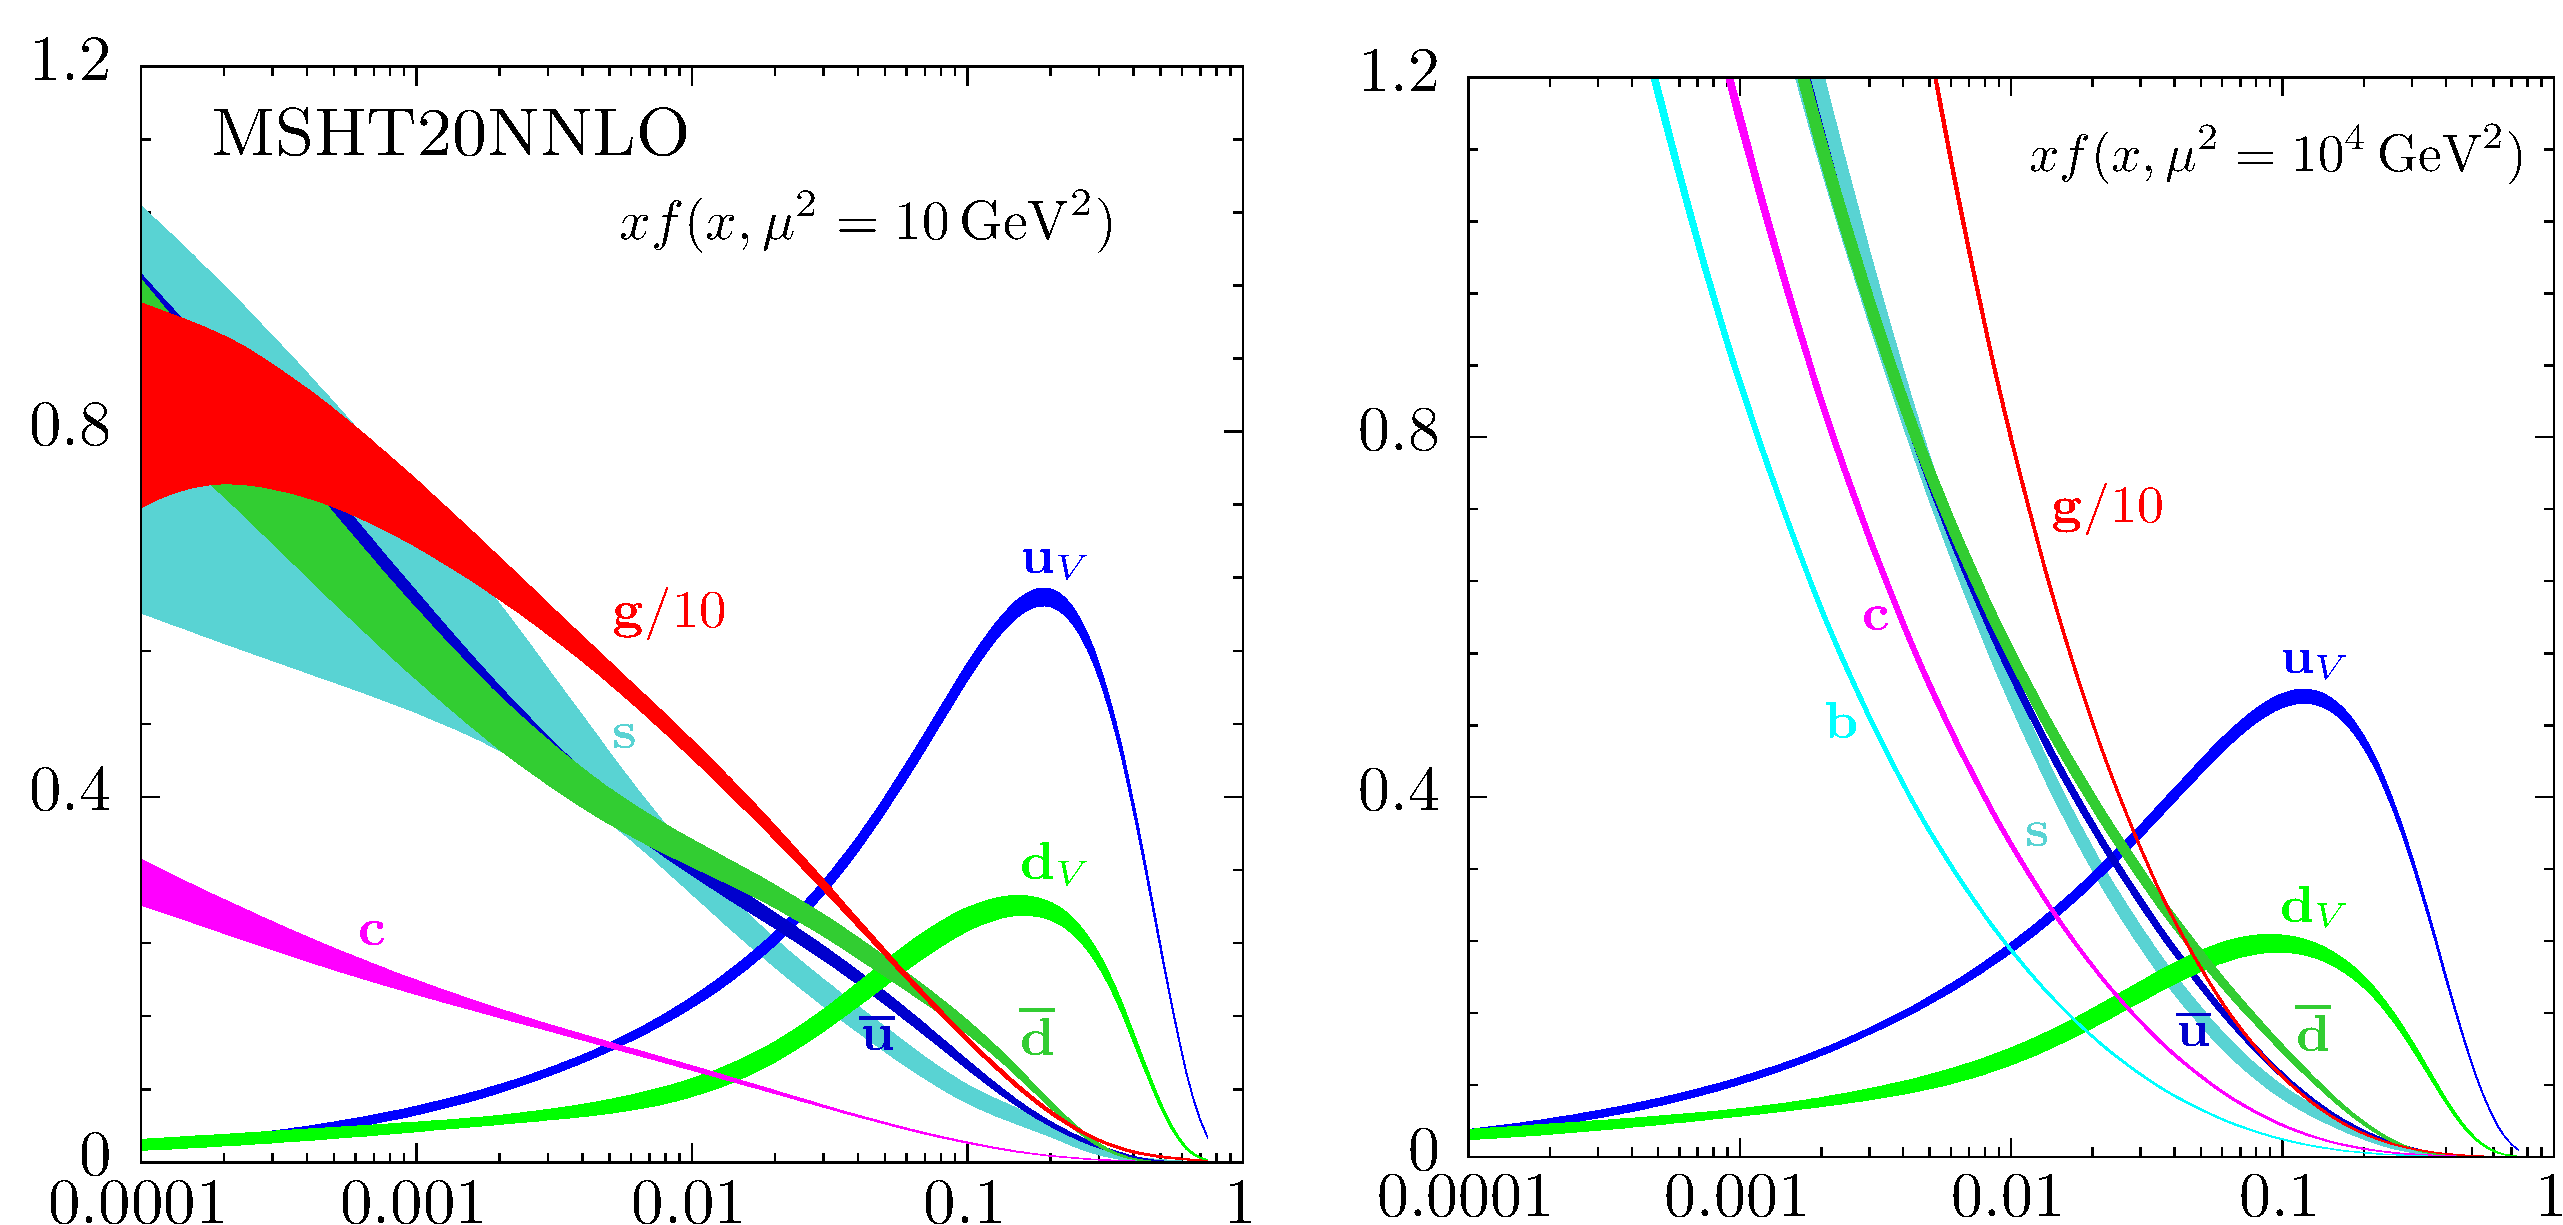
\includegraphics[width=1.0\textwidth]{msht_new.pdf}
\caption{\label{fig:PDF} The bands are $x$ times the unpolarized parton distributions $f(x)$ (where $f=u_v,d_v,\bar{u},\bar{d},s\approx\bar{s},c=\bar{c},b=\bar{b},g$) obtained in the NNLO MSHT20 global analysis at scales $\mu^2=10~\gev^2$ (left) and $\mu^2=10^4~\gev^2$, with $\alpha_s(M_Z^2)=0.118$. Cited from PDG.}
\end{figure}
\begin{enumerate}[1)]
    \item The production mechanism of Higgs at LHC is shown in following figure, 
    \begin{figure}
    \centering
    \includegraphics[width=1.1\textwidth]{feynman1.png}
    \caption{\label{fig:HiggsFeynman}Higgs production mechanism.}
    \end{figure}
    determine which one is the main process to produce Higgs.
    \item The production mechanism of top quark pair $t\bar{t}$ at collider is shown in following figure, 
    \begin{figure}
    \centering
    \includegraphics[width=1.1\textwidth]{feynman2.png}
    \caption{\label{fig:TopFeynman}Top quark production mechanism.}
    \end{figure}
    determine which one is the main process at LHC and Tevatron.
\end{enumerate}
\end{problem}

\begin{solution}
\begin{enumerate}[1)]
    \item For the gluon fusion, the momentum fraction is
    \begin{align}
        x=\frac{m_H}{\sqrt{s}}=\frac{125~\gev}{14~\tev}\approx=0.009\ ,
    \end{align}
    for the associated production and vector boson fusion, the momentum fraction is
    \begin{align}
        x=\frac{2m_q+m_H}{\sqrt{s}}=\frac{2m_q+(125~\gev) }{14~\tev}>0.009\ ,
    \end{align}
    according to the PDF with $\mu^2=10^4~\gev^2$, the contribution from gluon is much bigger than others at $x=0.009$, thus the vector-boson fusion has the less chance to proceed. With the increase of $x$, the gluon contribution becomes small, which means the chance of gluon fusion is bigger than associated production. Therefore, the gluon fusion is the main process to produce Higgs at LHC.
    \item At LHC, with the center-of-mass $\sqrt{s_1}=8~\tev$ and $\sqrt{s_2}=14~\tev$, the momentum fraction of producing a pair of top quarks is
    \begin{align}
        x_1=\frac{2m_t}{\sqrt{s_1}}=\frac{345~\gev}{8~\tev}\approx 0.043\ ;\quad
        x_2=\frac{2m_t}{\sqrt{s_2}}=\frac{345~\gev}{14~\tev}\approx 0.025\ ,
    \end{align}
    according to the PDF, the main contributor at $x_1=0.043$ or $x_2=0.025$ is the gluon, which means the main process to produce top quark pairs at LHC is the gluon channel. \\
    At Tevatron, with the center-of-mass $\sqrt{s}=2~\tev$, the momentum fraction of producing a pair of top quarks is
    \begin{align}
        x=\frac{2m_t}{\sqrt{s}}=\frac{345~\gev}{2~\tev}\approx 0.17\ ,
    \end{align}
    according to the PDF, the main contributor at $x=0.17$ is the quarks, which means the main process to produce top quark pairs at Tevatron is the quark channel.
\end{enumerate}
\end{solution}

\begin{problem}
In high-energy physics experiments, the production of quarks and gluons manifests as jets. For example, in the center of mass frame, when a high-energy electron-positron pair annihilates to produce a quark-antiquark pair, they will appear as two opposite jets. If one of the quarks radiates a hard gluon, this gluon carries away nearly half of the quark's energy, resulting in the quark, antiquark, and gluon fragmenting into three jets (which are detected as three jets emanating from a single point). This is known as the famous three-jet event. The significance of the three-jet event lies in its experimental confirmation of the objective existence of gluons.
\end{problem}

\chapter{Weak Interaction and the Electroweak Model}

\begin{problem}
    Based on your understanding, briefly summarize the key points of the universal Fermi $V-A$ low-energy effective theory of weak interactions, including its universality, the meaning of $V-A$, its low-energy effectiveness and limitations, the structure of leptons' charged current and quarks' charged current.
\end{problem}

\begin{solution}
    The universality means that for the beta decay, lepton decay and quark weak decay with $\Delta S=0/1$, they share the same coupling constant $G_{F}$. \par
    The $V-A$ means the charged weak current structure in the Lagrangian of weak interaction, that is
    \begin{align}
        J^{(+)}=\bar{\psi}_{l}\gamma^{\mu}(1-\gamma^5)\psi_{\nu_l}=2\bar{\psi}_{lL}\gamma^{\mu}\psi_{\nu_lL}\ ,
    \end{align}
    where the $\gamma^{\mu}$ represent vector current ($V$) and $\gamma^{\mu}\gamma^5$ represent axial current ($A$), it shows that only the left hand electron and neutrino are coupled together. \par
    The low-energy effectiveness shows that the Feimi $V-A$ theory is an effective theory to describe the weak interaction, while when the energy scale goes to and even larger than the mass of media boson, the cross-section of four fermions interaction would be divergent, which meas it breaks the unitary limitation.\par
    The structure of quarks' charged current (without considering the $c,b,t$ quarks) is
    \begin{align}
        J^{(-)}_{q}=\bar{u}\gamma^{\mu}(1-\gamma^5)(d\cos{\theta_C}+s\sin{\theta_C})\ ,
    \end{align}
    where $\theta_C$ is the Cabbibo angle.
\end{solution}

\begin{problem}
    What is the lepton number? What is the lepton number conservation? Pay attention to whether the lepton number is conserved in weak interactions.
\end{problem}

\begin{solution}
    Each generation leptons have their own lepton numbers, for the $e,\nu_e$ with $L_e=L_{\nu_e}=L_1=+1$, for the $\mu,\nu_{\mu}$ with $L_{\mu}=L_{\nu_{\mu}}=L_2=+1$, for the $\tau,\nu_{\tau}$ with $L_{\tau}=L_{\nu_{\tau}}=L_3=+1$. \par
    The lepton number conservation means each generation lepton numbers before and after a process should be the same individually, this is a universal conservation for all the interaction in Standard Model.
\end{solution}

\begin{problem}
    How do you understand the short range of weak interactions? What are the numbers of $M_W$ and $M_Z$? How are they related to the Fermi constant?
\end{problem}

\begin{solution}
    Compared to the Electromagnetic force, the weak force can be described by Yukawa potential
    \begin{align}
        V_W(r)=-\frac{\alpha_W}{r}e^{-m_Wr}\ ,
    \end{align}
    let $m_W\to\infty$, we have
    \begin{align}
        V_W(r)=-\frac{4\pi\alpha_W}{m_W^2}\delta^{(3)}(\mathbf{r})\ ,
    \end{align}
    which goes to the Fermi point interaction, assuming $\alpha_W\approx\alpha=1/137$, we have
    \begin{align}
        m_W=\sqrt{\frac{4\pi\alpha}{G_F}}\approx 100~\gevcs\ ,
    \end{align}
    the force range is
    \begin{align}
        L=\frac{1}{m_W}\approx 10^{-18}\rm m\ ,
    \end{align}
    which shows that the weak interaction range is short. \par
    The mass of $W^{\pm}$ is $M_{w}=80.4~\gevcs$ and of $Z^0$ is $M_{Z}=91.2~\gevcs$. Using Fermi constant $G_F$, the $M_{W}$ and $M_{Z}$ can be expressed as 
    \begin{align}
        M_{W}=2^{-5/4}\frac{g}{\sqrt{G_F}}\ ;\quad M_{Z}=2^{-5/4}\frac{\sqrt{g^2+g'^2}}{\sqrt{G_F}}\ ,
    \end{align}
    where $g$ and $g'$ are the coupling constant of $W_{\mu}$ and $B_{\mu}$.
\end{solution}

\begin{problem}
    Why does the neutrino have no its anti-partner? Why are neutrino and anti-neutrino associated by $CP$-parity? 
\end{problem}

\begin{solution}
    If the neutrino is massless, only the left hand neutrino and right hand anti-neutrino are existed. Particle and anti-particle is associated by $C$-parity, while the result of $C$-transformation of left hand neutrino is the left hand anti-neutrino, which is not existed. The only way connecting left hand neutrino and right hand anti-neutrino is $CP$-transformation, where $P$ transformes left hand to right hand and $C$ transformes neutrino to anti-neutrino.
\end{solution}

\begin{problem}
    What is the fundamental symmetry of the electroweak unification theory? What are the basic degrees of freedom (using the first-generation leptons as an example)? How are quarks represented as the basic degrees of freedom in the electroweak unification theory?
\end{problem}

\begin{solution}
    The basic symmetry is SU(2) $\otimes$ U(1). For the first generation of leptons, the left-handed neutrino and left-handed electron form a doublet representation of SU(2), while the right-handed electron is a singlet under SU(2). For quarks, the doublets of weak isospin SU(2) are formed by left-handed quarks $(u_L, d_L'), (c_L, s_L'), (t_L, b_L')$, where $d', s', b'$ are the weak eigenstates, which are combinations of the mass eigenstates $d,s,b$, indicating mixing between generations. The right-handed quarks are singlets under SU(2).
\end{solution}

\begin{problem}
    What is the Weinberg angle $\theta_W$? What is the neutral current? What is the relationship between them? How are the Weinberg angle $\theta_W$ defined by $M_W$, $M_Z$?
\end{problem}

\begin{solution}
    Weinberg angle $\theta_W$ is introduced by
    \begin{align}
        \begin{pmatrix}
            Z_{\mu} \\
            A_{\mu}
        \end{pmatrix}
        =
        \begin{pmatrix}
            \cos{\theta_W} & -\sin{\theta_W} \\
            \sin{\theta_W} & \cos{\theta_W}
        \end{pmatrix}
        \begin{pmatrix}
            W^3_{\mu} \\
            B_{\mu}
        \end{pmatrix}\ ,
    \end{align}
    where $Z_{\mu}$ and $A_{\mu}$ are the $Z^0$ boson field and photon field, $W^3_{\mu}$ is the third gauge field of SU(2) symmetry, and $B_{\mu}$ is the gauge field of U(1) symmetry. \par
    Neutral current is the current interacting with $Z^0$ boson, it can be written as (for the first generation lepton)
    \begin{align}
        J_{\text{NC}}=\frac{1}{2}\bar{\nu}_{eL}\gamma^{\mu}\nu_{eL}-\frac{1}{2}\bar{e}_L\gamma^{\mu}e_{L}+\sin^2{\theta_{W}}\bar{e}\gamma^{\mu}e\ ,
    \end{align}
    where $\theta_W$ is the Weinberg angle, when the kind of fermions is fixed, the neutral current is only determined by Weinberg angle.
\end{solution}

\begin{problem}
    What puzzle in weak interactions does the Cabibbo theory address? What problem is solved by the GIM mechanism? What is quark mixing? What is the physical meaning of the CKM matrix?
\end{problem}

\begin{solution}
    Before the Cabibbo theory, the strange number unchanged and changed charged current of hadrons seem to be described by the same theory, however, the coupling strength of this two kinds of process is different, that is $G'/G_{\beta}\approx 0.2$. Also, the the coupling of beta decay and muon decay is $G_{\beta}/G_{\mu}=0.98$, which is not consistent with each other. The Cabibbo theory assumes that there are mixing between $d$ and $s$ quark
    \begin{align}
        d'=\cos{\theta_C}d+\sin{\theta_C}s\ ,
    \end{align}
    as a result, the ratios of coupling are
    \begin{align}
        \frac{G_{\beta}}{G_{\mu}}=\cos{\theta_C}=0.977\ ;\quad\frac{G'}{G_{\beta}}=\frac{\sin{\theta_C}}{\cos{\theta_C}}\approx 0.2\ ,
    \end{align}
    which unifies the hadrons' weak decay and leptons' weak decay.\par
    The Cabibbo theory only allow the coupling between $d'$ and $u$ but no such coupling between $s'$ and $u$, which results in that there should be flavour changed neutral current, that is
    \begin{align}
        \bar{u}u+\bar{d'}d'=\bar{u}u+(\cos^2{\theta_C}\bar{d}d+\sin^2{\theta_C}\bar{s}s)+\sin{\theta_C}\cos{\theta_C}(\bar{s}d+\bar{d}s)\ ,
    \end{align}
    the third term gives the flavour changed neutral current.\par
    However, this kind of process is suppressed experimentally. To solve this problem, the GIM mechanism predicts the existence of charm quark ($c$) and it should be coupled to the $s'$, as a result, we have
    \begin{align}
        \bar{u}u+\bar{d'}d'+\bar{c}c+\bar{s'}s'=\bar{u}u+\bar{d}d+\bar{c}c+\bar{s}s\ ,
    \end{align}
    where the flavour changed neutral current is canceled.\par
    The quarks $q$, as the eigenstates of strong interaction, are able to interact with weak field. However, the eigenstates of weak interaction are $q'$, which are the mixture of quarks, and it can be expressed as
    \begin{align}
        \begin{pmatrix}
            d' \\
            s' \\
            b'
        \end{pmatrix}=
        \begin{pmatrix}
            V_{ud} & V_{us} & V_{ub} \\
            V_{cd} & V_{cs} & V_{cb} \\
            V_{td} & V_{ts} & V_{tb}
        \end{pmatrix}
        \begin{pmatrix}
            d \\
            s \\
            b
        \end{pmatrix}\ ,
    \end{align}
    the $3\times 3$ matrix is called Cabibbo-Kobayashi-Maskawa matrix.
\end{solution}

\begin{problem}
    What is spontaneous symmetry breaking? What problem is solved by the Higgs mechanism introduced in the electroweak interactions? How do the media bosons acquire masses? What is the Yukawa coupling? How do fermion acquire masses?
\end{problem}

\begin{solution}
    Although the Lagrangian of the system exhibits a certain symmetry, the selection of a specific vacuum state leads to the breaking of this symmetry. This mechanism is referred to as spontaneous symmetry breaking.\par
    As a gauge theory, the gauge bosons of electroweak theory should be massless, howvever, in fact, the media bosons of weak interaction $W$ and $Z$ are massive. Higgs mechanism introduces Higgs field, and Higgs field gives the $W$ and $Z$ masses.\par
    When we coupled the Higgs with $W_{\mu}$ and $B_{\mu}$, the kinematic term of Higgs field Lagrangian is
    \begin{align}
        \mathcal{L}_{\text{H}}=(D_{\mu}\Phi(x))^{\dagger}(D^{\mu}\Phi(x))\ ,
    \end{align}
    where $\Phi(x)$ is the Higgs field and $D_{\mu}$ is the covariant derivative
    \begin{align}
        D_{\mu}=\partial_{\mu}-igW^a_{\mu}\sigma_a/2-ig'B_{\mu}/2\ ,
    \end{align}
    thus the vacuum expected value of Higgs field is
    \begin{align}
        &\quad\langle 0|\Phi^{\dagger}|0\rangle(igW^a_{\mu}\sigma_a/2+ig'B_{\mu}/2)(-igW^a_{\mu}\sigma_a/2-ig'B_{\mu}/2)\rangle 0|\Phi|0\rangle \nonumber \\
        &=\frac{g^2\rho^2_0}{4}W^+_{\mu}W^{-\mu}+\frac{1}{2}\frac{(g^2+g'^2)\rho^2_0}{4}Z_{\mu}Z^{\mu} \nonumber \\
        &=m_WW^+_{\mu}W^{-\mu}+\frac{1}{2}m_Z Z_{\mu}Z^{\mu}\ ,
    \end{align}
    therefore, the Higgs field gives the mass of $W$ and $Z$ bosons.\par
    For the fermions, their masses are given by the Yukawa coupling with Higgs. Yukawa coupling refers to the coupling of spinor field and scalar field. For the electron, the Lagrangian is
    \begin{align}
        \mathcal{L}_{\text{Yukawa}}=-f_e\bar{e}_{R}\Phi^{\dagger}\begin{pmatrix}
            \nu_{eL} \\
            e_L
        \end{pmatrix}+h.c.\ ,
    \end{align}
    thus the vacuum expected value is
    \begin{align}
        &\quad -f_e[\bar{e}_{R}\langle 0|\Phi^{\dagger}|0\rangle\begin{pmatrix}
            \nu_{eL} \\
            e_L
        \end{pmatrix}+h.c.] \nonumber \\
        &=-\frac{f_e\rho_0}{\sqrt{2}}(\bar{e}_Re_L+\bar{e}_Le_R) \nonumber \\
        &=-\frac{f_e\rho_0}{\sqrt{2}}\bar{e}e \nonumber \\
        &=-m_e\bar{e}e\ ,
    \end{align}
    which accounts for the origin of the mass of electron.
\end{solution}

\begin{problem}
    Organize and familiarize yourself with various charged current weak processes mentioned in the lecture notes, such as beta decay and charged current weak processes involving strangeness change. Understand the characteristics of the initial and final state particles in neutral current weak processes and be able to accurately identify them.
\end{problem}

\begin{solution}
    The charged current is composed of different fermion fields, which couple to $W^{\pm}$. At the coupling vertex, the two fermions are particles within the same weak isospin SU(2) doublet. While, each term in the neutral current is composed of the same fermion field. The fermions can be quarks, charged leptons, or neutrinos, and the neutral current couples to the $Z^0$ field.
\end{solution}

\begin{problem}
    What does neutrino oscillation mean? How is the neutrino oscillation pattern determined in neutrino oscillation experiments? How are neutrino mixing angles measured?
\end{problem}

\begin{solution}
    Neutrino oscillation shows that neurtino is massive. The $\nu_e,\nu_{\mu}$ and $\nu_{\tau}$ are the eigenstates of weak interaction and they are composed of $\nu_1,\nu_2$ and $\nu_3$, which are the eigenstates of mass. The probability of $\nu_{\mu}$ transforming to $\nu_e$ is
    \begin{align}
        P(\nu_{\mu}\to\nu_e)=\sin^2{2\theta}\sin^2{\frac{1.27\Delta m^2L}{E}}\ ,
    \end{align}
    the oscillation pattern is determined by $\Delta m^2$ and mixing angle is determined by $\theta$.
\end{solution}

\begin{problem}
    The experiments conducted at the LHC represent the high-energy frontier of particle physics. The LHC is a hadron collider (proton-proton collisions), where high-energy physics processes can be considered to occur between partons.
    \begin{enumerate}[1)]
        \item Consider the LHC, where a heavy particle is formed by the fusion of two partons, each originating from one of the colliding protons. In the lowest-order approximation, neglecting the transverse momentum of the two partons, discuss the kinematics of the partons along the proton-proton collision direction.
        \item Describe the three production mechanisms of the Higgs boson at the LHC. Which one is the most dominant?
        \item Explain the mechanisms for producing top quark pairs at the LHC. Which one is the primary mechanism?
        \item List the mechanisms for single top quark production at a hadron collider (list as many as possible).
    \end{enumerate}
\end{problem}

\begin{solution}
    \begin{enumerate}[1)]
        \item Let the momenta of initial protons be $P_1$ and $P_2$, the momentum fractions of partons are $x_1$ and $x_2$, thus the invariant mass of the heavy particle is
        \begin{align}
            m_X^2=(x_1P_1+x_2P_2)^2=x_1^2P_1^2+x_2^2P_2^2+2x_1x_2P_1P_2\approx 2x_1x_2P_1P_2\ ,
        \end{align}
        where we have ignored the mass of proton when the center-of-mass energy is pretty high. For the energy and momentum of $X$, we have
        \begin{align}
            E_X&=x_1E_1+x_2E_2=x_1|\mathbf{P}_1|+x_2|\mathbf{P}_2|\ , \nonumber \\
            \mathbf{p}_X&=x_1\mathbf{P}_1+x_2\mathbf{P}_2\ .
        \end{align}
        \item The three production mechanism of Higgs at the LHC are shown blew, according to the parton model, the dominant process is gluon fusion.
        \begin{figure}
        \centering
        \includegraphics[width=1.1\textwidth]{feynman1.png}
        \caption{\label{fig:HiggsFeynman2}Higgs production mechanism.}
        \end{figure}
        \item The three production mechanism of top quark at the LHC are shown blew, according to the parton model, the dominant process is gluon channel.
        \begin{figure}
        \centering
        \includegraphics[width=1.1\textwidth]{feynman2.png}
        \caption{\label{fig:TopFeynman2}Top quark production mechanism.}
        \end{figure}
        \item The Feynman diagrams for single top quark production are shown blew.
        \begin{align*}
        \begin{fmffile}{complex-a}
        \begin{fmfgraph*}(120,75)
            \fmfstraight
            \fmfleft{i1}
            \fmfright{o1,o2,o3}
            \fmf{fermion,tension=3.6,label=$q$}{i1,w1}
            \fmf{zigzag,label=$W^+$}{w1,w2}
            \fmf{fermion,label=$q'$}{w1,o1}
            \fmf{fermion,tension=.6,label=$t$}{w2,o2}
            \fmf{fermion,label=$\bar{b}$}{o3,w2}
        \end{fmfgraph*}
        \end{fmffile}\quad
        \begin{fmffile}{complex-a}
        \begin{fmfgraph*}(120,75)
            \fmfstraight
            \fmfleft{i1,i2}
            \fmfright{o1,o2}
            \fmf{gluon,label=$g$}{i1,w1}
            \fmf{fermion,label=$b$}{i2,w1}
            \fmf{fermion,label=$b$}{w1,w2}
            \fmf{fermion,label=$t$}{w2,o2}
            \fmf{zigzag,label=$W^{-}$}{w2,o1}
        \end{fmfgraph*}
        \end{fmffile}\quad
        \begin{fmffile}{complex-a}
        \begin{fmfgraph*}(120,75)
            \fmfleft{i1,i2}
            \fmfright{o1,o2}
            \fmf{fermion,label=$e^-$}{i1,w1}
            \fmf{fermion,label=$e^+$}{w1,i2}
            \fmf{zigzag,label=$Z^0$}{w1,w2}
            \fmf{zigzag,label=$Z^0$}{w2,o2}
            \fmf{scalar,label=$H$}{w2,o1}
        \end{fmfgraph*}
        \end{fmffile}
        \end{align*}
    \end{enumerate}
\end{solution}

\begin{problem}
    China is planning to build a Circular Electron-Positron Collider (CEPC). Do you know the production mechanisms of the Higgs boson at the CEPC? It would be best to represent them using Feynman diagrams.
\end{problem}

\begin{solution}
    The Feynman diagrams of production mechanisms of the Higgs boson at the CEPC are shown blew.
    \begin{align*}
        \begin{fmffile}{complex-a}
        \begin{fmfgraph*}(120,75)
            \fmfleft{i1,i2}
            \fmfright{o1,o2,o3}
            \fmf{fermion,label=$e^-$}{i1,w1}
            \fmf{fermion,label=$e^+$}{w2,i2}
            \fmf{zigzag,label=$Z^0$}{w1,w3}
            \fmf{zigzag,label=$Z^0$}{w2,w3}
            \fmf{scalar,tension=.6,label=$H$}{w3,o2}
            \fmf{fermion,label=$\nu_{e}/e^-$}{w1,o1}
            \fmf{fermion,label=$\bar{\nu}_{e}/e^+$}{o3,w2}
        \end{fmfgraph*}
        \end{fmffile}\quad
        \begin{fmffile}{complex-a}
        \begin{fmfgraph*}(120,75)
            \fmfleft{i1,i2}
            \fmfright{o1,o2}
            \fmf{fermion,label=$q$}{i1,w1}
            \fmf{fermion,label=$\bar{q}'$}{w1,i2}
            \fmf{zigzag,label=$W^+$}{w1,w2}
            \fmf{fermion,label=$t$}{w2,o1}
            \fmf{fermion,label=$\bar{b}$}{o2,w2}
        \end{fmfgraph*}
        \end{fmffile}
    \end{align*}
\end{solution}
\end{document}